% Options for packages loaded elsewhere
\PassOptionsToPackage{unicode}{hyperref}
\PassOptionsToPackage{hyphens}{url}
%
\documentclass[
]{book}
\usepackage{amsmath,amssymb}
\usepackage{lmodern}
\usepackage{iftex}
\ifPDFTeX
  \usepackage[T1]{fontenc}
  \usepackage[utf8]{inputenc}
  \usepackage{textcomp} % provide euro and other symbols
\else % if luatex or xetex
  \usepackage{unicode-math}
  \defaultfontfeatures{Scale=MatchLowercase}
  \defaultfontfeatures[\rmfamily]{Ligatures=TeX,Scale=1}
\fi
% Use upquote if available, for straight quotes in verbatim environments
\IfFileExists{upquote.sty}{\usepackage{upquote}}{}
\IfFileExists{microtype.sty}{% use microtype if available
  \usepackage[]{microtype}
  \UseMicrotypeSet[protrusion]{basicmath} % disable protrusion for tt fonts
}{}
\makeatletter
\@ifundefined{KOMAClassName}{% if non-KOMA class
  \IfFileExists{parskip.sty}{%
    \usepackage{parskip}
  }{% else
    \setlength{\parindent}{0pt}
    \setlength{\parskip}{6pt plus 2pt minus 1pt}}
}{% if KOMA class
  \KOMAoptions{parskip=half}}
\makeatother
\usepackage{xcolor}
\usepackage{color}
\usepackage{fancyvrb}
\newcommand{\VerbBar}{|}
\newcommand{\VERB}{\Verb[commandchars=\\\{\}]}
\DefineVerbatimEnvironment{Highlighting}{Verbatim}{commandchars=\\\{\}}
% Add ',fontsize=\small' for more characters per line
\usepackage{framed}
\definecolor{shadecolor}{RGB}{248,248,248}
\newenvironment{Shaded}{\begin{snugshade}}{\end{snugshade}}
\newcommand{\AlertTok}[1]{\textcolor[rgb]{0.94,0.16,0.16}{#1}}
\newcommand{\AnnotationTok}[1]{\textcolor[rgb]{0.56,0.35,0.01}{\textbf{\textit{#1}}}}
\newcommand{\AttributeTok}[1]{\textcolor[rgb]{0.77,0.63,0.00}{#1}}
\newcommand{\BaseNTok}[1]{\textcolor[rgb]{0.00,0.00,0.81}{#1}}
\newcommand{\BuiltInTok}[1]{#1}
\newcommand{\CharTok}[1]{\textcolor[rgb]{0.31,0.60,0.02}{#1}}
\newcommand{\CommentTok}[1]{\textcolor[rgb]{0.56,0.35,0.01}{\textit{#1}}}
\newcommand{\CommentVarTok}[1]{\textcolor[rgb]{0.56,0.35,0.01}{\textbf{\textit{#1}}}}
\newcommand{\ConstantTok}[1]{\textcolor[rgb]{0.00,0.00,0.00}{#1}}
\newcommand{\ControlFlowTok}[1]{\textcolor[rgb]{0.13,0.29,0.53}{\textbf{#1}}}
\newcommand{\DataTypeTok}[1]{\textcolor[rgb]{0.13,0.29,0.53}{#1}}
\newcommand{\DecValTok}[1]{\textcolor[rgb]{0.00,0.00,0.81}{#1}}
\newcommand{\DocumentationTok}[1]{\textcolor[rgb]{0.56,0.35,0.01}{\textbf{\textit{#1}}}}
\newcommand{\ErrorTok}[1]{\textcolor[rgb]{0.64,0.00,0.00}{\textbf{#1}}}
\newcommand{\ExtensionTok}[1]{#1}
\newcommand{\FloatTok}[1]{\textcolor[rgb]{0.00,0.00,0.81}{#1}}
\newcommand{\FunctionTok}[1]{\textcolor[rgb]{0.00,0.00,0.00}{#1}}
\newcommand{\ImportTok}[1]{#1}
\newcommand{\InformationTok}[1]{\textcolor[rgb]{0.56,0.35,0.01}{\textbf{\textit{#1}}}}
\newcommand{\KeywordTok}[1]{\textcolor[rgb]{0.13,0.29,0.53}{\textbf{#1}}}
\newcommand{\NormalTok}[1]{#1}
\newcommand{\OperatorTok}[1]{\textcolor[rgb]{0.81,0.36,0.00}{\textbf{#1}}}
\newcommand{\OtherTok}[1]{\textcolor[rgb]{0.56,0.35,0.01}{#1}}
\newcommand{\PreprocessorTok}[1]{\textcolor[rgb]{0.56,0.35,0.01}{\textit{#1}}}
\newcommand{\RegionMarkerTok}[1]{#1}
\newcommand{\SpecialCharTok}[1]{\textcolor[rgb]{0.00,0.00,0.00}{#1}}
\newcommand{\SpecialStringTok}[1]{\textcolor[rgb]{0.31,0.60,0.02}{#1}}
\newcommand{\StringTok}[1]{\textcolor[rgb]{0.31,0.60,0.02}{#1}}
\newcommand{\VariableTok}[1]{\textcolor[rgb]{0.00,0.00,0.00}{#1}}
\newcommand{\VerbatimStringTok}[1]{\textcolor[rgb]{0.31,0.60,0.02}{#1}}
\newcommand{\WarningTok}[1]{\textcolor[rgb]{0.56,0.35,0.01}{\textbf{\textit{#1}}}}
\usepackage{longtable,booktabs,array}
\usepackage{calc} % for calculating minipage widths
% Correct order of tables after \paragraph or \subparagraph
\usepackage{etoolbox}
\makeatletter
\patchcmd\longtable{\par}{\if@noskipsec\mbox{}\fi\par}{}{}
\makeatother
% Allow footnotes in longtable head/foot
\IfFileExists{footnotehyper.sty}{\usepackage{footnotehyper}}{\usepackage{footnote}}
\makesavenoteenv{longtable}
\usepackage{graphicx}
\makeatletter
\def\maxwidth{\ifdim\Gin@nat@width>\linewidth\linewidth\else\Gin@nat@width\fi}
\def\maxheight{\ifdim\Gin@nat@height>\textheight\textheight\else\Gin@nat@height\fi}
\makeatother
% Scale images if necessary, so that they will not overflow the page
% margins by default, and it is still possible to overwrite the defaults
% using explicit options in \includegraphics[width, height, ...]{}
\setkeys{Gin}{width=\maxwidth,height=\maxheight,keepaspectratio}
% Set default figure placement to htbp
\makeatletter
\def\fps@figure{htbp}
\makeatother
\setlength{\emergencystretch}{3em} % prevent overfull lines
\providecommand{\tightlist}{%
  \setlength{\itemsep}{0pt}\setlength{\parskip}{0pt}}
\setcounter{secnumdepth}{5}
\usepackage{booktabs}
\usepackage[utf8]{inputenc}
\usepackage[english,russian]{babel}
\usepackage{fontspec}
\setmainfont[Ligatures=TeX,
             Path=font/,
             BoldFont=brillb,
             ItalicFont=brilli,
             BoldItalicFont=brillbi]{brill}
\setmonofont[Scale=0.7,
             Path=font/]{iosevka-regular}

\usepackage{longtable}
\usepackage[bf,singlelinecheck=off]{caption}

\usepackage{framed,color}
\definecolor{shadecolor}{RGB}{248,248,248}

\renewcommand{\textfraction}{0.05}
\renewcommand{\topfraction}{0.8}
\renewcommand{\bottomfraction}{0.8}
\renewcommand{\floatpagefraction}{0.75}

\let\oldhref\href
\renewcommand{\href}[2]{#2\footnote{\url{#1}}}
  \makeatletter
  \newenvironment{kframe}{%
    \medskip{}
    \setlength{\fboxsep}{.8em}
    \def\at@end@of@kframe{}%
    \ifinner\ifhmode%
    \def\at@end@of@kframe{\end{minipage}}%
    \begin{minipage}{\columnwidth}%
    \fi\fi%
    \def\FrameCommand##1{\hskip\@totalleftmargin \hskip-\fboxsep
    \colorbox{shadecolor}{##1}\hskip-\fboxsep
      % There is no \\@totalrightmargin, so:
        \hskip-\linewidth \hskip-\@totalleftmargin \hskip\columnwidth}%
    \MakeFramed {\advance\hsize-\width
      \@totalleftmargin\z@ \linewidth\hsize
      \@setminipage}}%
  {\par\unskip\endMakeFramed%
    \at@end@of@kframe}
  \makeatother
  
  \makeatletter
  \@ifundefined{Shaded}{
  }{\renewenvironment{Shaded}{\begin{kframe}}{\end{kframe}}}
  \makeatother
  
  \newenvironment{rmdblock}[1]
  {
    \begin{itemize}
    \renewcommand{\labelitemi}{
      \raisebox{-.7\height}[0pt][0pt]{
        {\setkeys{Gin}{width=3em,keepaspectratio}\includegraphics{images/#1}}
        }
        }
        \setlength{\fboxsep}{1em}
        \begin{kframe}
        \item
      }
      {
        \end{kframe}
        \end{itemize}
      }
      \newenvironment{rmdtask}
      {\begin{rmdblock}{task}}
      {\end{rmdblock}}
      
      \usepackage{makeidx}
      \makeindex
      
      \urlstyle{tt}
      
      \usepackage{amsthm}
      \makeatletter
      \def\thm@space@setup{%
        \thm@preskip=8pt plus 2pt minus 4pt
        \thm@postskip=\thm@preskip
      }
      \makeatother
\ifLuaTeX
  \usepackage{selnolig}  % disable illegal ligatures
\fi
\usepackage[]{natbib}
\bibliographystyle{apalike}
\IfFileExists{bookmark.sty}{\usepackage{bookmark}}{\usepackage{hyperref}}
\IfFileExists{xurl.sty}{\usepackage{xurl}}{} % add URL line breaks if available
\urlstyle{same} % disable monospaced font for URLs
\hypersetup{
  pdftitle={Анализ данных для лингвистов},
  pdfauthor={Г. А. Мороз},
  hidelinks,
  pdfcreator={LaTeX via pandoc}}

\title{Анализ данных для лингвистов}
\author{Г. А. Мороз}
\date{}

\begin{document}
\maketitle

{
\setcounter{tocdepth}{1}
\tableofcontents
}
\hypertarget{ux43e-ux43aux443ux440ux441ux435}{%
\chapter{О курсе}\label{ux43e-ux43aux443ux440ux441ux435}}

Материалы для курса Анализа данных для лингвистов, Школа лингвистики НИУ ВШЭ.

\begin{itemize}
\tightlist
\item
  вместо первой лекции можно посмотреть \href{https://youtu.be/HmLcBJnfipk}{запись лекции 2021.01.13}
\item
  вместо второй лекции можно посмотреть \href{https://youtu.be/V_c_K_wBMuY}{запись лекции 2021.01.15}
\item
  вместо третей лекции можно посмотреть \href{https://youtu.be/cRc5z9F3XNw}{запись лекции 2021.01.20}
\item
  вместо четвертой лекции можно посмотреть \href{https://youtu.be/zj-1-invsGM}{запись лекции 2021.01.22}
\item
  вместо пятой лекции можно посмотреть \href{https://www.youtube.com/watch?v=2YRAdMLT4N0\&list=PL_HB2SrKjmMJ-dUBtXUSQBZxRftJJX5uL\&index=5}{запись лекции 2021.01.27}
\item
  вместо шестой лекции можно посмотреть \href{https://www.youtube.com/watch?v=FA-_Qbpmb6s\&list=PL_HB2SrKjmMJ-dUBtXUSQBZxRftJJX5uL\&index=6}{запись лекции 2021.01.29}
\item
  вместо седьмой лекции можно посмотреть \href{https://youtu.be/DkNnGeJT2K0}{запись лекции 2021.02.03}
\item
  вместо восьмой лекции можно посмотреть \href{https://youtu.be/c2mej30JnRM}{запись лекции 2021.02.05}
\item
  вместо девятой лекции можно посмотреть \href{https://youtu.be/9ltNRMQmt0U}{запись лекции 2021.02.10}
\item
  вместо десятой лекции можно посмотреть \href{https://youtu.be/zCG_edAziVk}{запись лекции 2021.02.12}
\item
  вместо одиннадцатой лекции можно посмотреть \href{https://youtu.be/6bERf7DMvfg}{запись лекции 2021.02.19}
\item
  вместо двеннадцатой лекции можно посмотреть \href{https://youtu.be/I80UaVOmpxY}{запись лекции 2021.02.24}
\item
  вместо триннадцатой и четырнадцатой лекций можно посмотреть вот эти видео: \href{https://youtu.be/_IltMx042DE}{часть 1}, \href{https://youtu.be/1qbk5dATogc}{часть 2}
\item
  вместо пятнадцатой лекции можно посмотреть \href{https://www.youtube.com/watch?v=mIhT4y4FigY\&list=PL_HB2SrKjmMJ-dUBtXUSQBZxRftJJX5uL\&index=12}{запись лекции 2021.03.03}
\item
  вместо шестнадцатой лекции можно посмотреть
  \href{https://www.youtube.com/watch?v=mIhT4y4FigY\&list=PL_HB2SrKjmMJ-dUBtXUSQBZxRftJJX5uL\&index=12}{запись лекции 2021.03.05} и
  \href{https://www.youtube.com/watch?v=m06AOJBU9Bo\&list=PL_HB2SrKjmMJ-dUBtXUSQBZxRftJJX5uL\&index=11}{другую} и
  \href{https://www.youtube.com/watch?v=XkEm4SHcYbg\&list=PL_HB2SrKjmMJ-dUBtXUSQBZxRftJJX5uL\&index=13}{третью},
\item
  вместо шестнадцатой лекции можно посмотреть вот это \href{https://youtu.be/a75VjnY-w0s}{видео}.
\end{itemize}

\hypertarget{ux438ux441ux43fux43eux43bux44cux437ux443ux435ux43cux44bux435-ux43fux430ux43aux435ux442ux44b}{%
\section{Используемые пакеты}\label{ux438ux441ux43fux43eux43bux44cux437ux443ux435ux43cux44bux435-ux43fux430ux43aux435ux442ux44b}}

\begin{Shaded}
\begin{Highlighting}[]
\FunctionTok{packageVersion}\NormalTok{(}\StringTok{"tidyverse"}\NormalTok{)}
\end{Highlighting}
\end{Shaded}

\begin{verbatim}
## [1] '1.3.2'
\end{verbatim}

\begin{Shaded}
\begin{Highlighting}[]
\FunctionTok{packageVersion}\NormalTok{(}\StringTok{"fitdistrplus"}\NormalTok{)}
\end{Highlighting}
\end{Shaded}

\begin{verbatim}
## [1] '1.1.8'
\end{verbatim}

\begin{Shaded}
\begin{Highlighting}[]
\FunctionTok{packageVersion}\NormalTok{(}\StringTok{"mixtools"}\NormalTok{)}
\end{Highlighting}
\end{Shaded}

\begin{verbatim}
## [1] '2.0.0'
\end{verbatim}

\begin{Shaded}
\begin{Highlighting}[]
\FunctionTok{packageVersion}\NormalTok{(}\StringTok{"lme4"}\NormalTok{)}
\end{Highlighting}
\end{Shaded}

\begin{verbatim}
## [1] '1.1.31'
\end{verbatim}

\begin{Shaded}
\begin{Highlighting}[]
\FunctionTok{packageVersion}\NormalTok{(}\StringTok{"lmerTest"}\NormalTok{)}
\end{Highlighting}
\end{Shaded}

\begin{verbatim}
## [1] '3.1.3'
\end{verbatim}

\begin{Shaded}
\begin{Highlighting}[]
\FunctionTok{packageVersion}\NormalTok{(}\StringTok{"car"}\NormalTok{)}
\end{Highlighting}
\end{Shaded}

\begin{verbatim}
## [1] '3.1.1'
\end{verbatim}

\begin{Shaded}
\begin{Highlighting}[]
\FunctionTok{packageVersion}\NormalTok{(}\StringTok{"pscl"}\NormalTok{)}
\end{Highlighting}
\end{Shaded}

\begin{verbatim}
## [1] '1.5.5'
\end{verbatim}

\begin{Shaded}
\begin{Highlighting}[]
\FunctionTok{packageVersion}\NormalTok{(}\StringTok{"nnet"}\NormalTok{)}
\end{Highlighting}
\end{Shaded}

\begin{verbatim}
## [1] '7.3.18'
\end{verbatim}

\begin{Shaded}
\begin{Highlighting}[]
\FunctionTok{packageVersion}\NormalTok{(}\StringTok{"MASS"}\NormalTok{)}
\end{Highlighting}
\end{Shaded}

\begin{verbatim}
## [1] '7.3.58'
\end{verbatim}

\begin{Shaded}
\begin{Highlighting}[]
\FunctionTok{packageVersion}\NormalTok{(}\StringTok{"ggeffects"}\NormalTok{)}
\end{Highlighting}
\end{Shaded}

\begin{verbatim}
## [1] '1.1.4'
\end{verbatim}

\begin{Shaded}
\begin{Highlighting}[]
\FunctionTok{packageVersion}\NormalTok{(}\StringTok{"brms"}\NormalTok{)}
\end{Highlighting}
\end{Shaded}

\begin{verbatim}
## [1] '2.18.0'
\end{verbatim}

\begin{Shaded}
\begin{Highlighting}[]
\FunctionTok{packageVersion}\NormalTok{(}\StringTok{"tidybayes"}\NormalTok{)}
\end{Highlighting}
\end{Shaded}

\begin{verbatim}
## [1] '3.0.2'
\end{verbatim}

\hypertarget{ux434ux43eux43cux430ux448ux43dux438ux435-ux437ux430ux434ux430ux43dux438ux44f}{%
\section{Домашние задания}\label{ux434ux43eux43cux430ux448ux43dux438ux435-ux437ux430ux434ux430ux43dux438ux44f}}

\begin{itemize}
\tightlist
\item
  домашнее задание к лекции 16.01.2023:

  \begin{itemize}
  \tightlist
  \item
    вспомните пожалуйста, условные вероятности, формулу Байеса и при каких условиях ее применяют;
  \item
    посмотрите освежающие материалы про \href{http://setosa.io/conditional/}{условную вероятность} и \href{https://www.youtube.com/watch?v=HZGCoVF3YvM}{формулу Байеса}.
  \end{itemize}
\end{itemize}

\hypertarget{ux440ux430ux441ux43fux440ux435ux434ux435ux43bux435ux43dux438ux44f}{%
\chapter{Распределения}\label{ux440ux430ux441ux43fux440ux435ux434ux435ux43bux435ux43dux438ux44f}}

\begin{Shaded}
\begin{Highlighting}[]
\FunctionTok{library}\NormalTok{(tidyverse)}
\end{Highlighting}
\end{Shaded}

\hypertarget{ux440ux430ux441ux43fux440ux435ux434ux435ux43bux435ux43dux438ux44f-ux432-r}{%
\section{Распределения в R}\label{ux440ux430ux441ux43fux440ux435ux434ux435ux43bux435ux43dux438ux44f-ux432-r}}

В R встроено какое-то количество известных распределений. Все они представлены четырьмя функциями:

\begin{itemize}
\tightlist
\item
  \texttt{d...} (функция плотности, probability density function),
\item
  \texttt{p...} (функция распределения, cumulative distribution function) --- интеграл площади под кривой от начала до указанной квантили
\item
  \texttt{q...} (обратная функции распределения, inverse cumulative distribution function) --- значение \emph{p}-той квантили распределения
\item
  и \texttt{r...} (рандомные числа из заданного распределения).
\end{itemize}

Рассмотрим все это на примере нормального распределения.

\begin{Shaded}
\begin{Highlighting}[]
\FunctionTok{tibble}\NormalTok{(}\AttributeTok{x =} \DecValTok{1}\SpecialCharTok{:}\DecValTok{100}\NormalTok{,}
       \AttributeTok{PDF =} \FunctionTok{dnorm}\NormalTok{(}\AttributeTok{x =}\NormalTok{ x, }\AttributeTok{mean =} \DecValTok{50}\NormalTok{, }\AttributeTok{sd =} \DecValTok{10}\NormalTok{)) }\SpecialCharTok{\%\textgreater{}\%} 
  \FunctionTok{ggplot}\NormalTok{(}\FunctionTok{aes}\NormalTok{(x, PDF))}\SpecialCharTok{+}
  \FunctionTok{geom\_point}\NormalTok{()}\SpecialCharTok{+}
  \FunctionTok{geom\_line}\NormalTok{()}\SpecialCharTok{+}
  \FunctionTok{labs}\NormalTok{(}\AttributeTok{title =} \StringTok{"PDF нормального распределения (μ = 50, sd = 10)"}\NormalTok{)}
\end{Highlighting}
\end{Shaded}

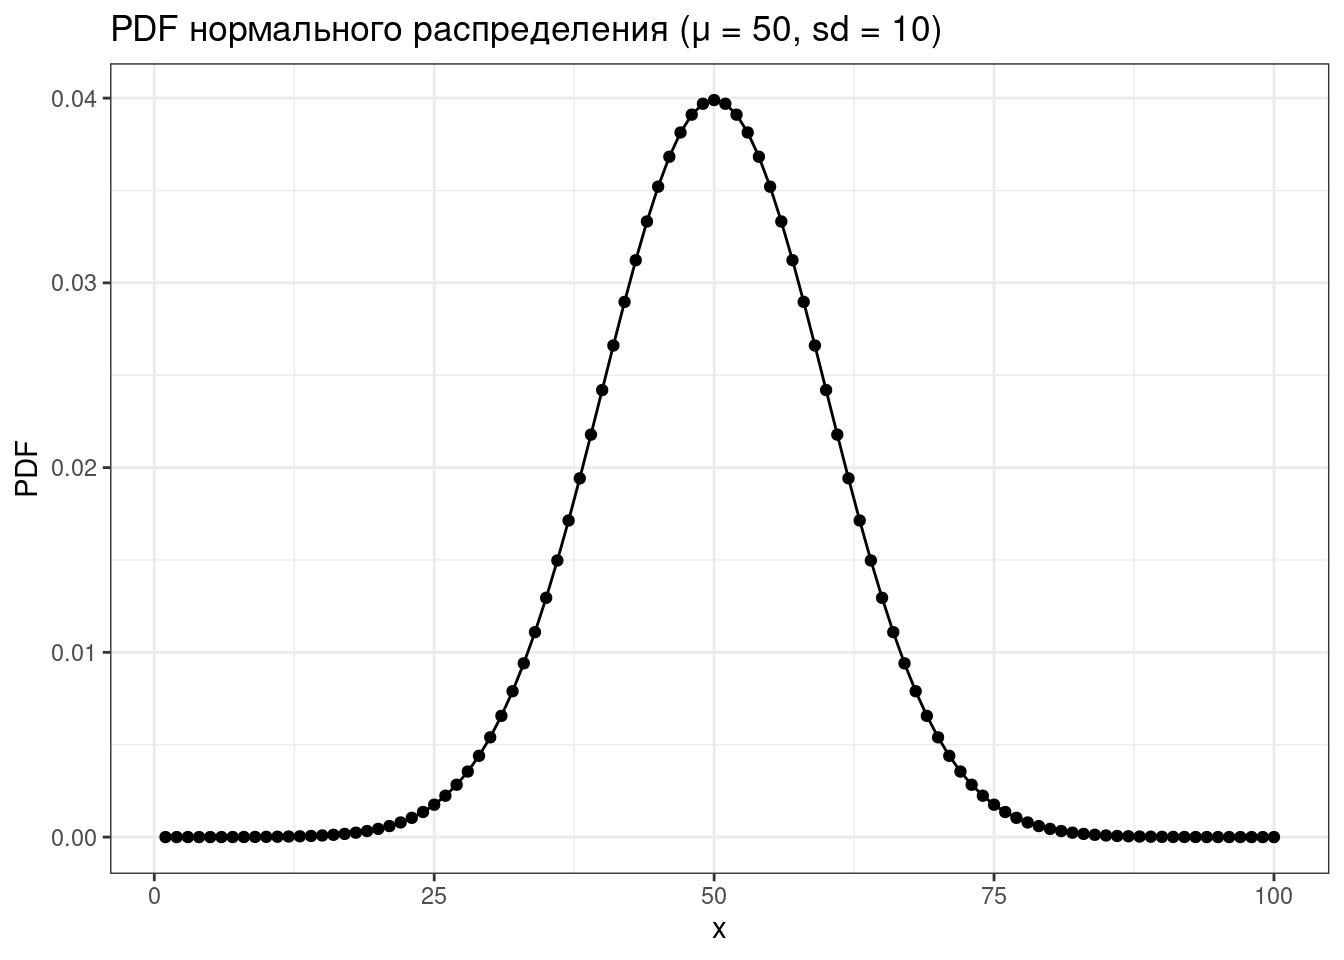
\includegraphics{da4l_files/figure-latex/unnamed-chunk-3-1.pdf}

\begin{Shaded}
\begin{Highlighting}[]
\FunctionTok{tibble}\NormalTok{(}\AttributeTok{x =} \DecValTok{1}\SpecialCharTok{:}\DecValTok{100}\NormalTok{,}
       \AttributeTok{CDF =} \FunctionTok{pnorm}\NormalTok{(x, }\AttributeTok{mean =} \DecValTok{50}\NormalTok{, }\AttributeTok{sd =} \DecValTok{10}\NormalTok{)) }\SpecialCharTok{\%\textgreater{}\%} 
  \FunctionTok{ggplot}\NormalTok{(}\FunctionTok{aes}\NormalTok{(x, CDF))}\SpecialCharTok{+}
  \FunctionTok{geom\_point}\NormalTok{()}\SpecialCharTok{+}
  \FunctionTok{geom\_line}\NormalTok{()}\SpecialCharTok{+}
  \FunctionTok{labs}\NormalTok{(}\AttributeTok{title =} \StringTok{"CDF нормального распределения (μ = 50, sd = 10)"}\NormalTok{)}
\end{Highlighting}
\end{Shaded}

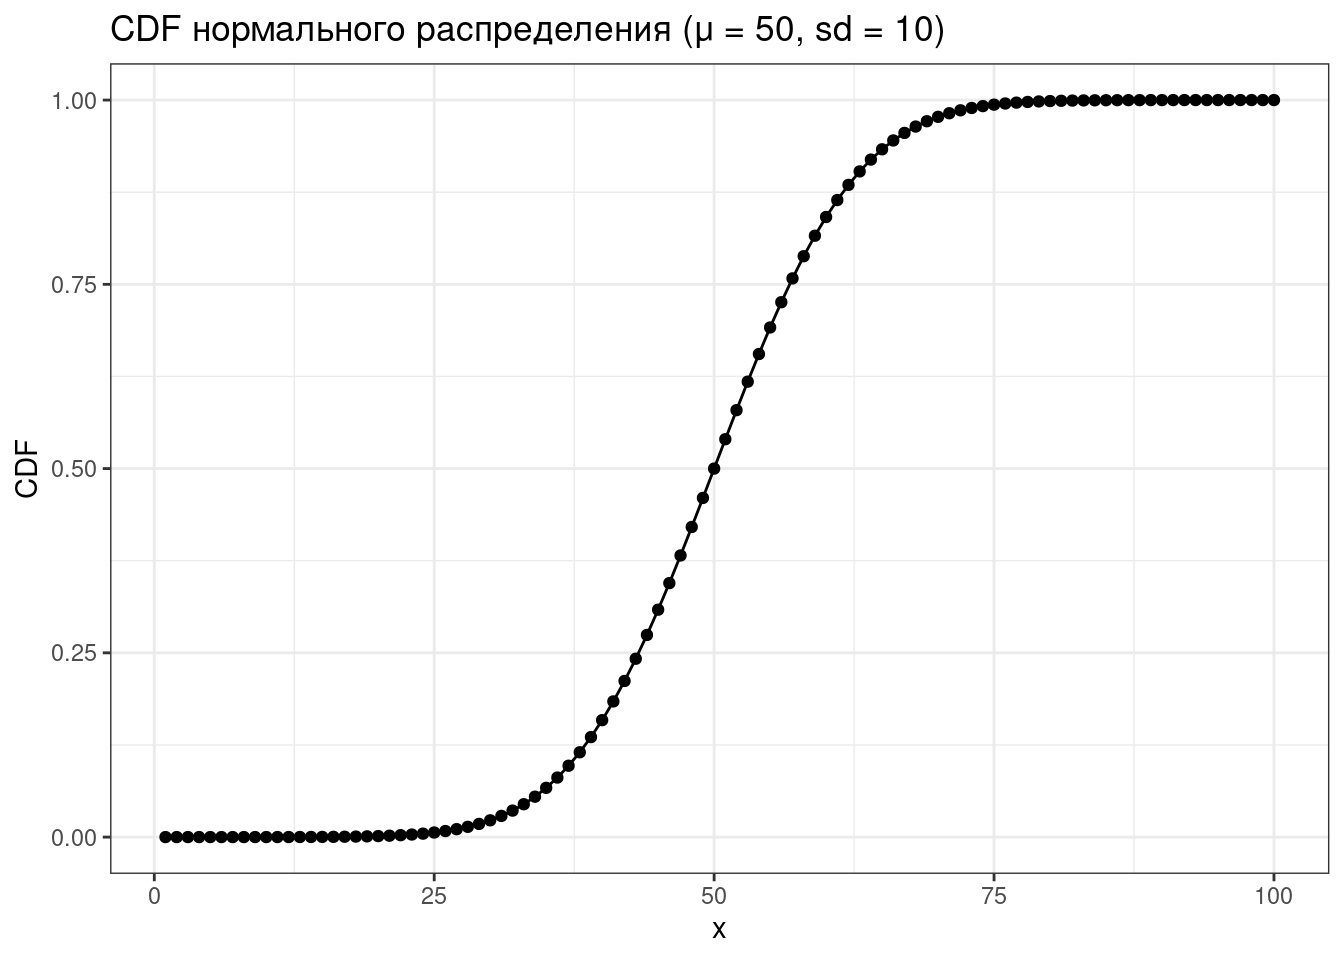
\includegraphics{da4l_files/figure-latex/unnamed-chunk-3-2.pdf}

\begin{Shaded}
\begin{Highlighting}[]
\FunctionTok{tibble}\NormalTok{(}\AttributeTok{quantiles =} \FunctionTok{seq}\NormalTok{(}\DecValTok{0}\NormalTok{, }\DecValTok{1}\NormalTok{, }\AttributeTok{by =} \FloatTok{0.01}\NormalTok{),}
       \AttributeTok{value =} \FunctionTok{qnorm}\NormalTok{(quantiles, }\AttributeTok{mean =} \DecValTok{50}\NormalTok{, }\AttributeTok{sd =} \DecValTok{10}\NormalTok{)) }\SpecialCharTok{\%\textgreater{}\%} 
  \FunctionTok{ggplot}\NormalTok{(}\FunctionTok{aes}\NormalTok{(quantiles, value))}\SpecialCharTok{+}
  \FunctionTok{geom\_point}\NormalTok{()}\SpecialCharTok{+}
  \FunctionTok{geom\_line}\NormalTok{()}\SpecialCharTok{+}
  \FunctionTok{labs}\NormalTok{(}\AttributeTok{title =} \StringTok{"inverse CDF нормального распределения (μ = 50, sd = 10)"}\NormalTok{)}
\end{Highlighting}
\end{Shaded}

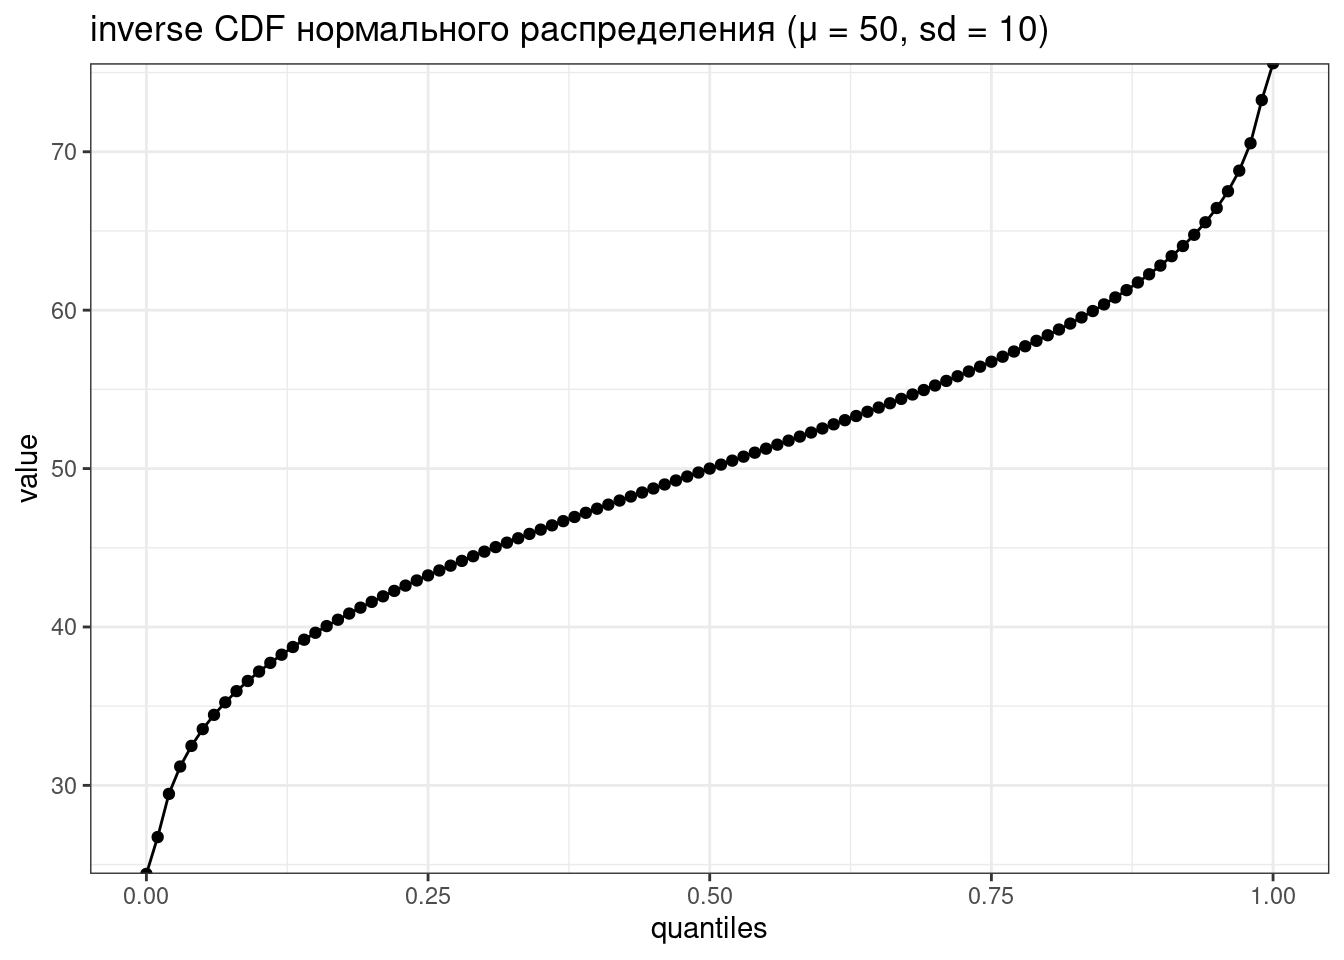
\includegraphics{da4l_files/figure-latex/unnamed-chunk-3-3.pdf}

\begin{Shaded}
\begin{Highlighting}[]
\FunctionTok{tibble}\NormalTok{(}\AttributeTok{sample =} \FunctionTok{rnorm}\NormalTok{(}\DecValTok{100}\NormalTok{, }\AttributeTok{mean =} \DecValTok{50}\NormalTok{, }\AttributeTok{sd =} \DecValTok{10}\NormalTok{)) }\SpecialCharTok{\%\textgreater{}\%} 
  \FunctionTok{ggplot}\NormalTok{(}\FunctionTok{aes}\NormalTok{(sample))}\SpecialCharTok{+}
  \FunctionTok{geom\_histogram}\NormalTok{()}\SpecialCharTok{+}
  \FunctionTok{labs}\NormalTok{(}\AttributeTok{title =} \StringTok{"выборка нормально распределенных чисел (μ = 50, sd = 10)"}\NormalTok{)}
\end{Highlighting}
\end{Shaded}

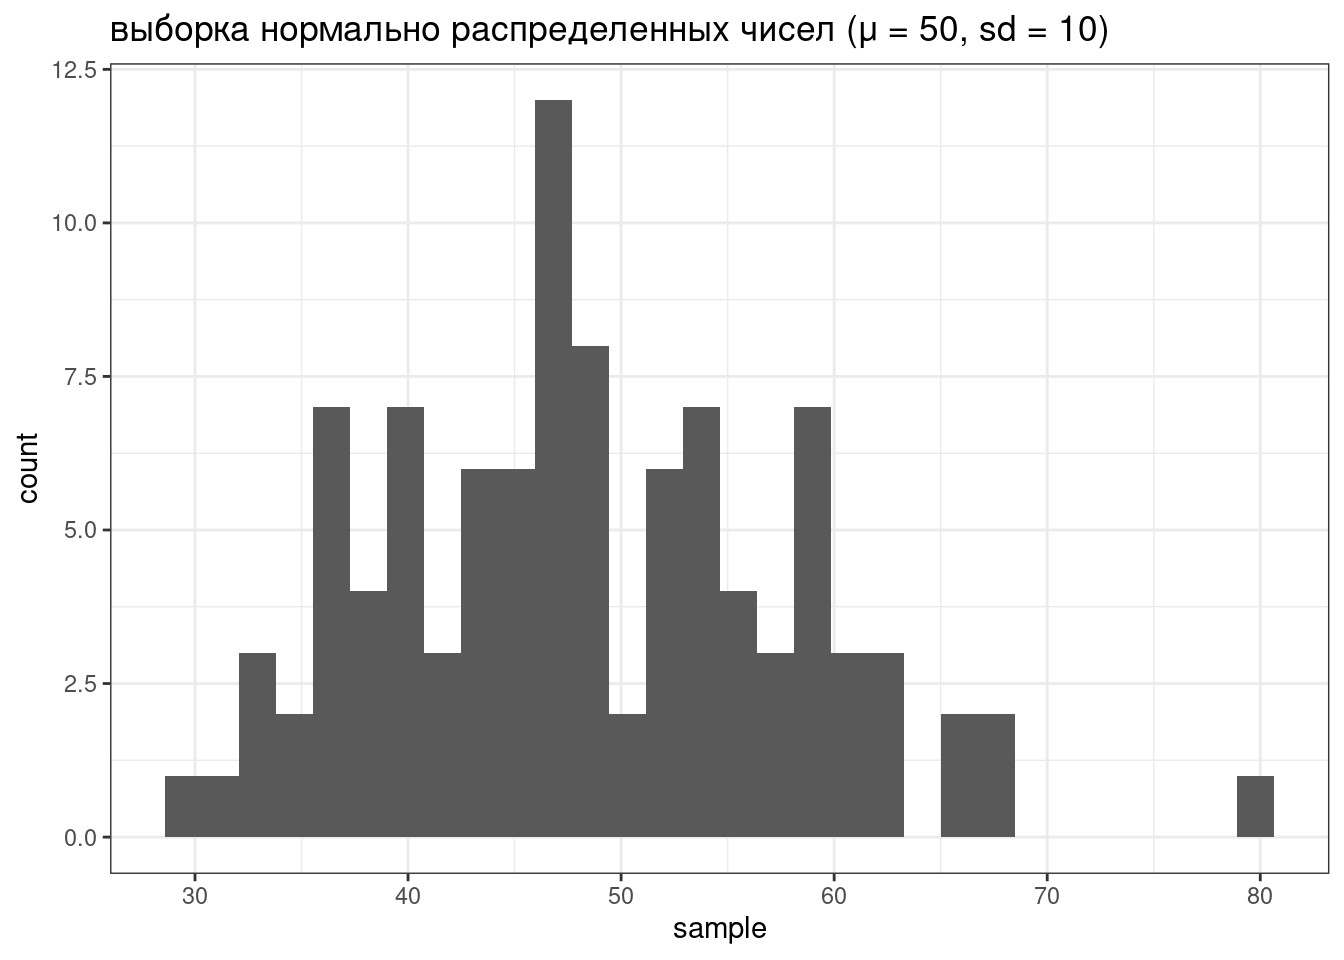
\includegraphics{da4l_files/figure-latex/unnamed-chunk-3-4.pdf}

Если не использовать \texttt{set.seed()}, то результат работы рандомизатора нельзя будет повторить.

\begin{rmdtask}
Какое значение имеет 25\% квантиль нормального распределения со средним
в 20 и стандартным отклонением 90? Ответ округлите до трех знаков после
запятой.
\end{rmdtask}

\begin{rmdtask}
Данные из базы данных фонетических инвентарей PHOIBLE {[}@phoible{]},
достаточно сильно упрощая, можно описать нормальным распределением со
средним 35 фонем и стандартным отклонением 13. Если мы ничего не знаем
про язык, оцените с какой вероятностью, согласно этой модели произвольно
взятый язык окажется в промежутке между 25 и 50 фонемами? Ответ
округлите до трех знаков после запятой.
\end{rmdtask}

\begin{rmdtask}
Какие есть недостатки у модели из предыдущего задания?
\end{rmdtask}

\hypertarget{ux434ux438ux441ux43aux440ux435ux442ux43dux44bux435-ux43fux435ux440ux435ux43cux435ux43dux43dux44bux435}{%
\section{Дискретные переменные}\label{ux434ux438ux441ux43aux440ux435ux442ux43dux44bux435-ux43fux435ux440ux435ux43cux435ux43dux43dux44bux435}}

\hypertarget{ux431ux438ux43dux43eux43cux438ux430ux43bux44cux43dux43eux435-ux440ux430ux441ux43fux440ux435ux434ux435ux43bux435ux43dux438ux435}{%
\subsection{Биномиальное распределение}\label{ux431ux438ux43dux43eux43cux438ux430ux43bux44cux43dux43eux435-ux440ux430ux441ux43fux440ux435ux434ux435ux43bux435ux43dux438ux435}}

Биномиальное распределение --- распределение количетсва успехов эксперементов Бернулли из \emph{n} попыток с вероятностью успеха \emph{p}.

\[P(k | n, p) = \frac{n!}{k!(n-k)!} \times p^k \times (1-p)^{n-k} =  {n \choose k} \times p^k \times (1-p)^{n-k}\]
\[ 0 \leq p \leq 1; n, k > 0\]

\begin{Shaded}
\begin{Highlighting}[]
\FunctionTok{tibble}\NormalTok{(}\AttributeTok{x =} \DecValTok{0}\SpecialCharTok{:}\DecValTok{50}\NormalTok{,}
       \AttributeTok{density =} \FunctionTok{dbinom}\NormalTok{(}\AttributeTok{x =}\NormalTok{ x, }\AttributeTok{size =} \DecValTok{50}\NormalTok{, }\AttributeTok{prob =} \FloatTok{0.16}\NormalTok{)) }\SpecialCharTok{\%\textgreater{}\%} 
  \FunctionTok{ggplot}\NormalTok{(}\FunctionTok{aes}\NormalTok{(x, density))}\SpecialCharTok{+}
  \FunctionTok{geom\_point}\NormalTok{()}\SpecialCharTok{+}
  \FunctionTok{geom\_line}\NormalTok{()}\SpecialCharTok{+}
  \FunctionTok{labs}\NormalTok{(}\AttributeTok{title =} \StringTok{"Биномиальное распределение p = 0.16, n = 50"}\NormalTok{)}
\end{Highlighting}
\end{Shaded}

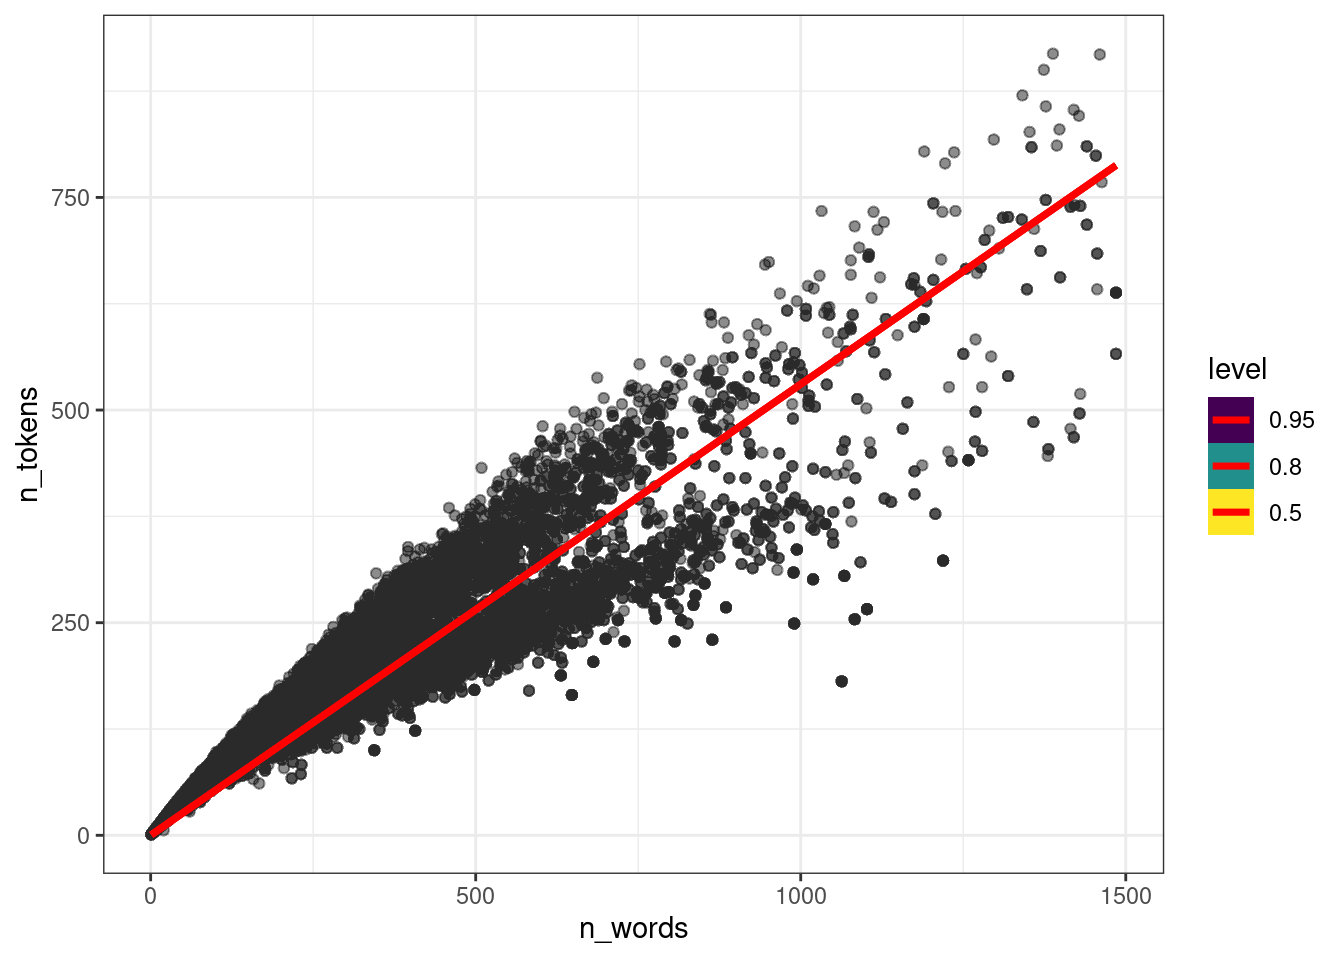
\includegraphics{da4l_files/figure-latex/unnamed-chunk-10-1.pdf}

\begin{rmdtask}
Немного упрощая данные из статьи {[}@rosenbach03: 394{]}, можно сказать
что носители британского английского предпочитают \emph{s}-генитив
(90\%) \emph{of}-генитиву (10\%). Какова вероятность, согласно этим
данным, что в интервью британского актера из 118 контекстов будет 102
\emph{s}-генитивов? Ответ округлите до трёх ИЛИ МЕНЕЕ знаков после
запятой.
\end{rmdtask}

\begin{rmdtask}
А какое значение количества \emph{s}-генитивов наиболее ожидаемо,
согласно этой модели?
\end{rmdtask}

\hypertarget{ux433ux435ux43eux43cux435ux442ux440ux438ux447ux435ux441ux43aux43eux435-ux440ux430ux441ux43fux440ux435ux434ux435ux43bux435ux43dux438ux435}{%
\subsection{Геометрическое распределение}\label{ux433ux435ux43eux43cux435ux442ux440ux438ux447ux435ux441ux43aux43eux435-ux440ux430ux441ux43fux440ux435ux434ux435ux43bux435ux43dux438ux435}}

Геометрическое распределение --- распределение количетсва эксперементов Бернулли с вероятностью успеха \emph{p} до первого успеха.

\[P(k | p) = (1-p)^k\times p\]
\[k\in\{1, 2, \dots\}\]

\begin{Shaded}
\begin{Highlighting}[]
\FunctionTok{tibble}\NormalTok{(}\AttributeTok{x =} \DecValTok{0}\SpecialCharTok{:}\DecValTok{50}\NormalTok{,}
       \AttributeTok{density =} \FunctionTok{dgeom}\NormalTok{(}\AttributeTok{x =}\NormalTok{ x, }\AttributeTok{prob =} \FloatTok{0.16}\NormalTok{)) }\SpecialCharTok{\%\textgreater{}\%} 
  \FunctionTok{ggplot}\NormalTok{(}\FunctionTok{aes}\NormalTok{(x, density))}\SpecialCharTok{+}
  \FunctionTok{geom\_point}\NormalTok{()}\SpecialCharTok{+}
  \FunctionTok{geom\_line}\NormalTok{()}\SpecialCharTok{+}
  \FunctionTok{labs}\NormalTok{(}\AttributeTok{title =} \StringTok{"Геометрическое распределение p = 0.16, n = 50"}\NormalTok{)}
\end{Highlighting}
\end{Shaded}

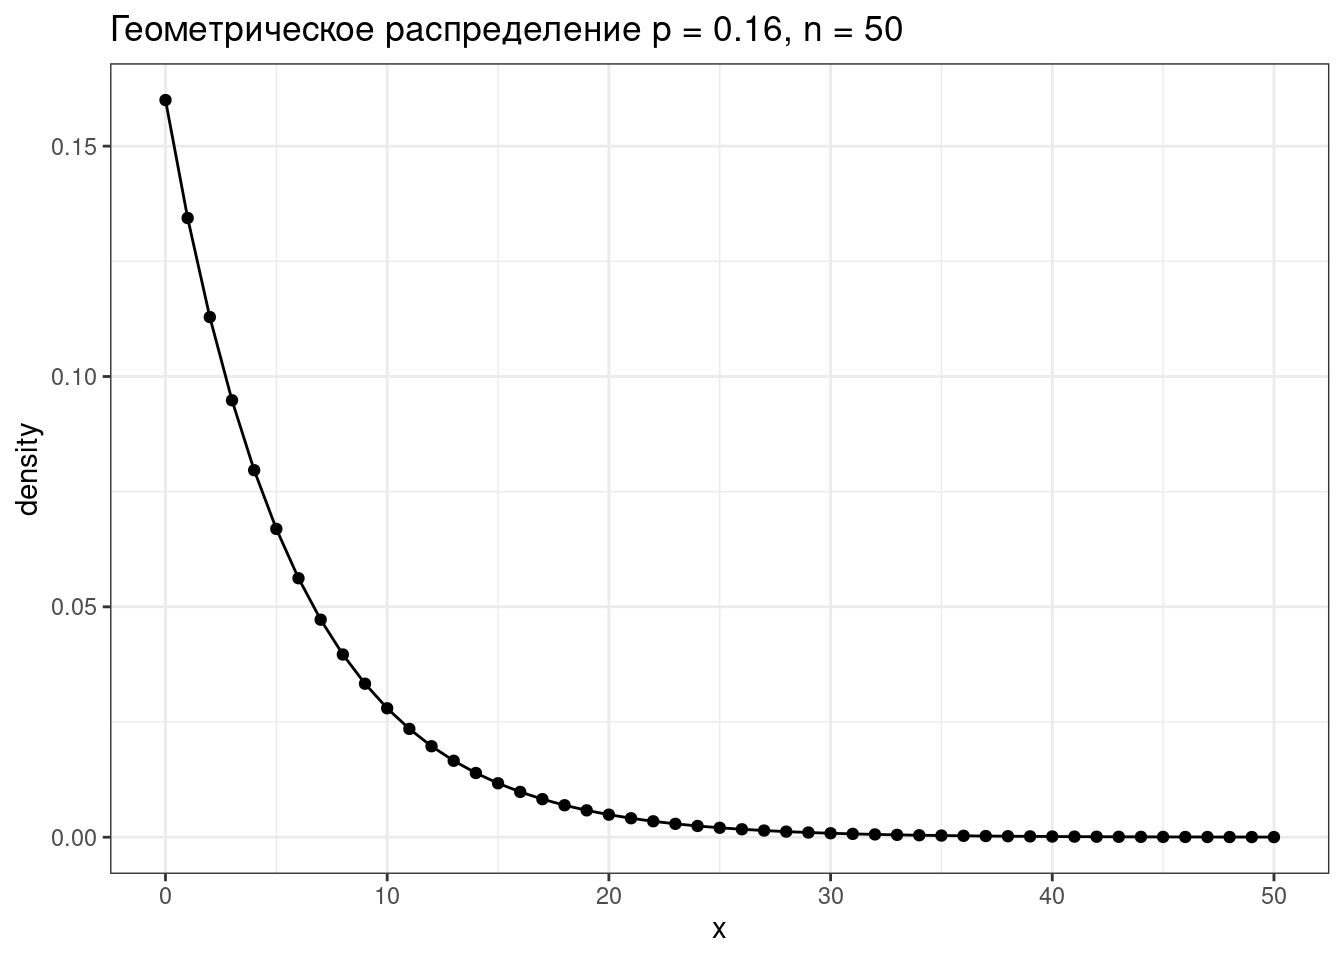
\includegraphics{da4l_files/figure-latex/unnamed-chunk-15-1.pdf}

\begin{rmdtask}
Приняв модель из {[}@rosenbach03: 394{]}, какова вероятность, что в
интервью с британским актером первый \emph{of}-генитив будет третьим по
счету?
\end{rmdtask}

\hypertarget{ux440ux430ux441ux43fux440ux435ux434ux435ux43bux435ux43dux438ux435-ux43fux443ux430ux441ux441ux43eux43dux430}{%
\subsection{Распределение Пуассона}\label{ux440ux430ux441ux43fux440ux435ux434ux435ux43bux435ux43dux438ux435-ux43fux443ux430ux441ux441ux43eux43dux430}}

Распределение дискретной переменной, обозначающей количество случаев \(k\) некоторого события, которое происходит с некоторой заданной частотой \(\lambda\).

\[P(\lambda) = \frac{e^{-\lambda}\times\lambda^k}{k!}\]

\begin{Shaded}
\begin{Highlighting}[]
\FunctionTok{tibble}\NormalTok{(}\AttributeTok{k =} \DecValTok{0}\SpecialCharTok{:}\DecValTok{50}\NormalTok{,}
       \AttributeTok{density =} \FunctionTok{dpois}\NormalTok{(}\AttributeTok{x =}\NormalTok{ k, }\AttributeTok{lambda =} \DecValTok{5}\NormalTok{)) }\SpecialCharTok{\%\textgreater{}\%} 
  \FunctionTok{ggplot}\NormalTok{(}\FunctionTok{aes}\NormalTok{(k, density))}\SpecialCharTok{+}
  \FunctionTok{geom\_point}\NormalTok{()}\SpecialCharTok{+}
  \FunctionTok{geom\_line}\NormalTok{()}\SpecialCharTok{+}
  \FunctionTok{labs}\NormalTok{(}\AttributeTok{title =} \StringTok{"Распределение Пуассона с параметром λ = 5"}\NormalTok{)}
\end{Highlighting}
\end{Shaded}

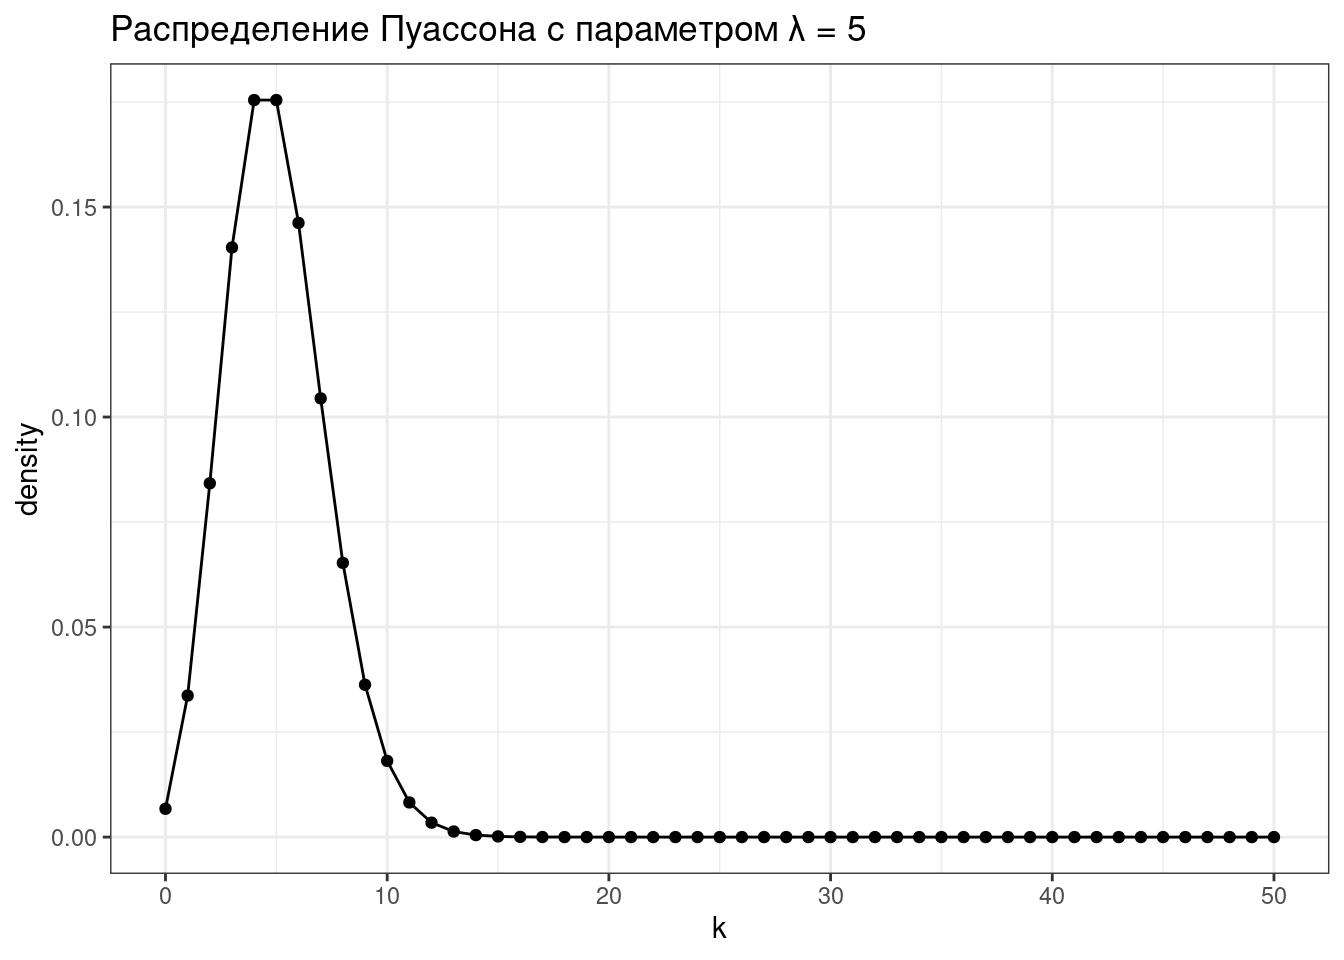
\includegraphics{da4l_files/figure-latex/unnamed-chunk-18-1.pdf}

Параметр \(\lambda\) в модели Пуассона одновременно является и средним, и дисперсией.

Попробуем воспользоваться распределением Пуассона для моделирования количества слогов в андийском языке. Количество слогов -- это всегда натуральное число (т. е. не бывает 2.5 слогов, не бывает -3 слогов и т. д., но в теории может быть 0 слогов), так что модель Пуассона здесь применима. Согласно модели Пуассона все слова независимо друг от друга получают сколько-то слогов согласно распределению Пуассона. Посмотрим на данные:

\begin{Shaded}
\begin{Highlighting}[]
\NormalTok{andic\_syllables }\OtherTok{\textless{}{-}} \FunctionTok{read\_csv}\NormalTok{(}\StringTok{"https://raw.githubusercontent.com/agricolamz/2021\_da4l/master/data/andic\_syllables.csv"}\NormalTok{) }

\NormalTok{andic\_syllables }\SpecialCharTok{\%\textgreater{}\%} 
  \FunctionTok{ggplot}\NormalTok{(}\FunctionTok{aes}\NormalTok{(n\_syllables, count))}\SpecialCharTok{+}
  \FunctionTok{geom\_col}\NormalTok{()}\SpecialCharTok{+}
  \FunctionTok{facet\_wrap}\NormalTok{(}\SpecialCharTok{\textasciitilde{}}\NormalTok{language, }\AttributeTok{scales =} \StringTok{"free"}\NormalTok{)}
\end{Highlighting}
\end{Shaded}

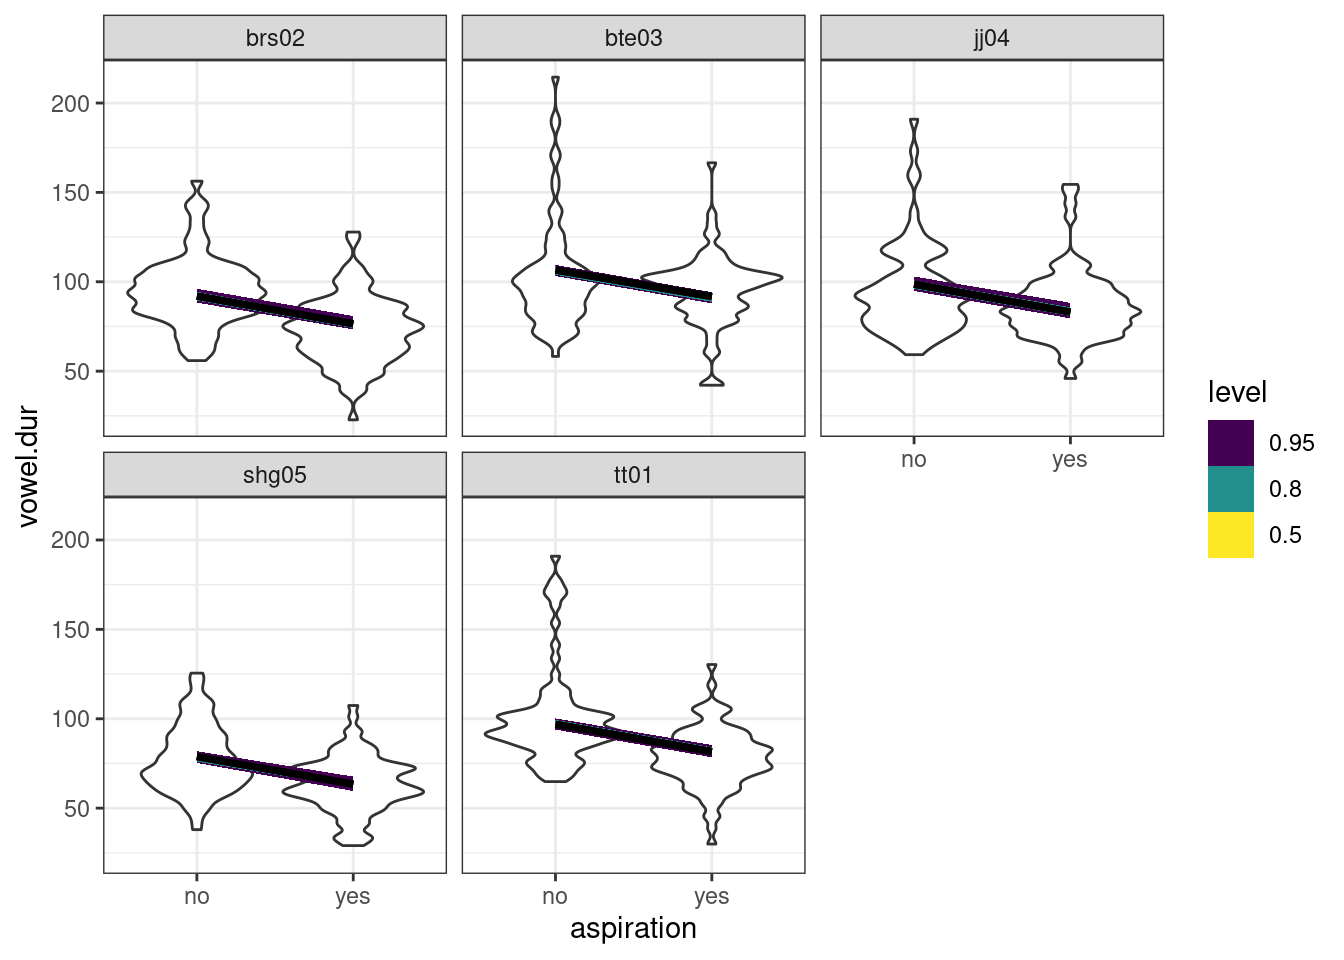
\includegraphics{da4l_files/figure-latex/unnamed-chunk-19-1.pdf}

Птичка напела (мы научимся узнавать, откуда птичка это знает на следующем занятии), что андийские данные можно описать при помощи распределения Пуассона с параметром \(\lambda\) = 2.783.

\begin{Shaded}
\begin{Highlighting}[]
\NormalTok{andic\_syllables }\SpecialCharTok{\%\textgreater{}\%} 
  \FunctionTok{filter}\NormalTok{(language }\SpecialCharTok{==} \StringTok{"Andi"}\NormalTok{) }\SpecialCharTok{\%\textgreater{}\%} 
  \FunctionTok{rename}\NormalTok{(}\AttributeTok{observed =}\NormalTok{ count) }\SpecialCharTok{\%\textgreater{}\%} 
  \FunctionTok{mutate}\NormalTok{(}\AttributeTok{predicted =} \FunctionTok{dpois}\NormalTok{(n\_syllables, }\AttributeTok{lambda =} \FloatTok{2.783}\NormalTok{)}\SpecialCharTok{*}\FunctionTok{sum}\NormalTok{(observed)) }\SpecialCharTok{\%\textgreater{}\%} 
  \FunctionTok{pivot\_longer}\NormalTok{(}\AttributeTok{names\_to =} \StringTok{"type"}\NormalTok{, }\AttributeTok{values\_to =} \StringTok{"value"}\NormalTok{, }\AttributeTok{cols =} \FunctionTok{c}\NormalTok{(observed, predicted)) }\SpecialCharTok{\%\textgreater{}\%} 
  \FunctionTok{ggplot}\NormalTok{(}\FunctionTok{aes}\NormalTok{(n\_syllables, value, }\AttributeTok{fill =}\NormalTok{ type))}\SpecialCharTok{+}
  \FunctionTok{geom\_col}\NormalTok{(}\AttributeTok{position =} \StringTok{"dodge"}\NormalTok{)}
\end{Highlighting}
\end{Shaded}

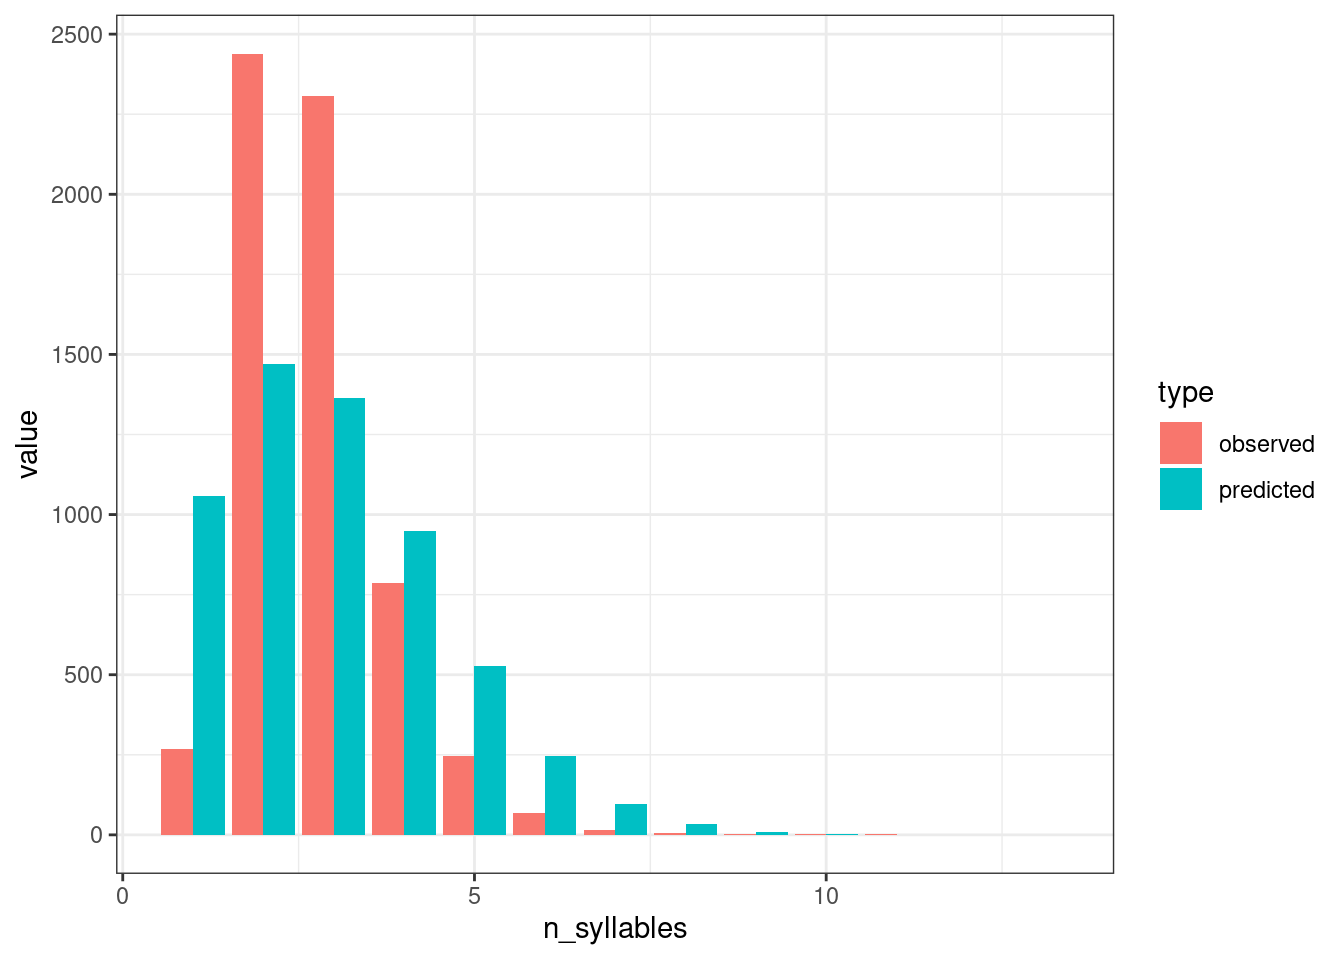
\includegraphics{da4l_files/figure-latex/unnamed-chunk-21-1.pdf}

\begin{rmdtask}
На графиках ниже представлены предсказания трех Пуассоновских моделей,
какая кажется лучше?
\end{rmdtask}

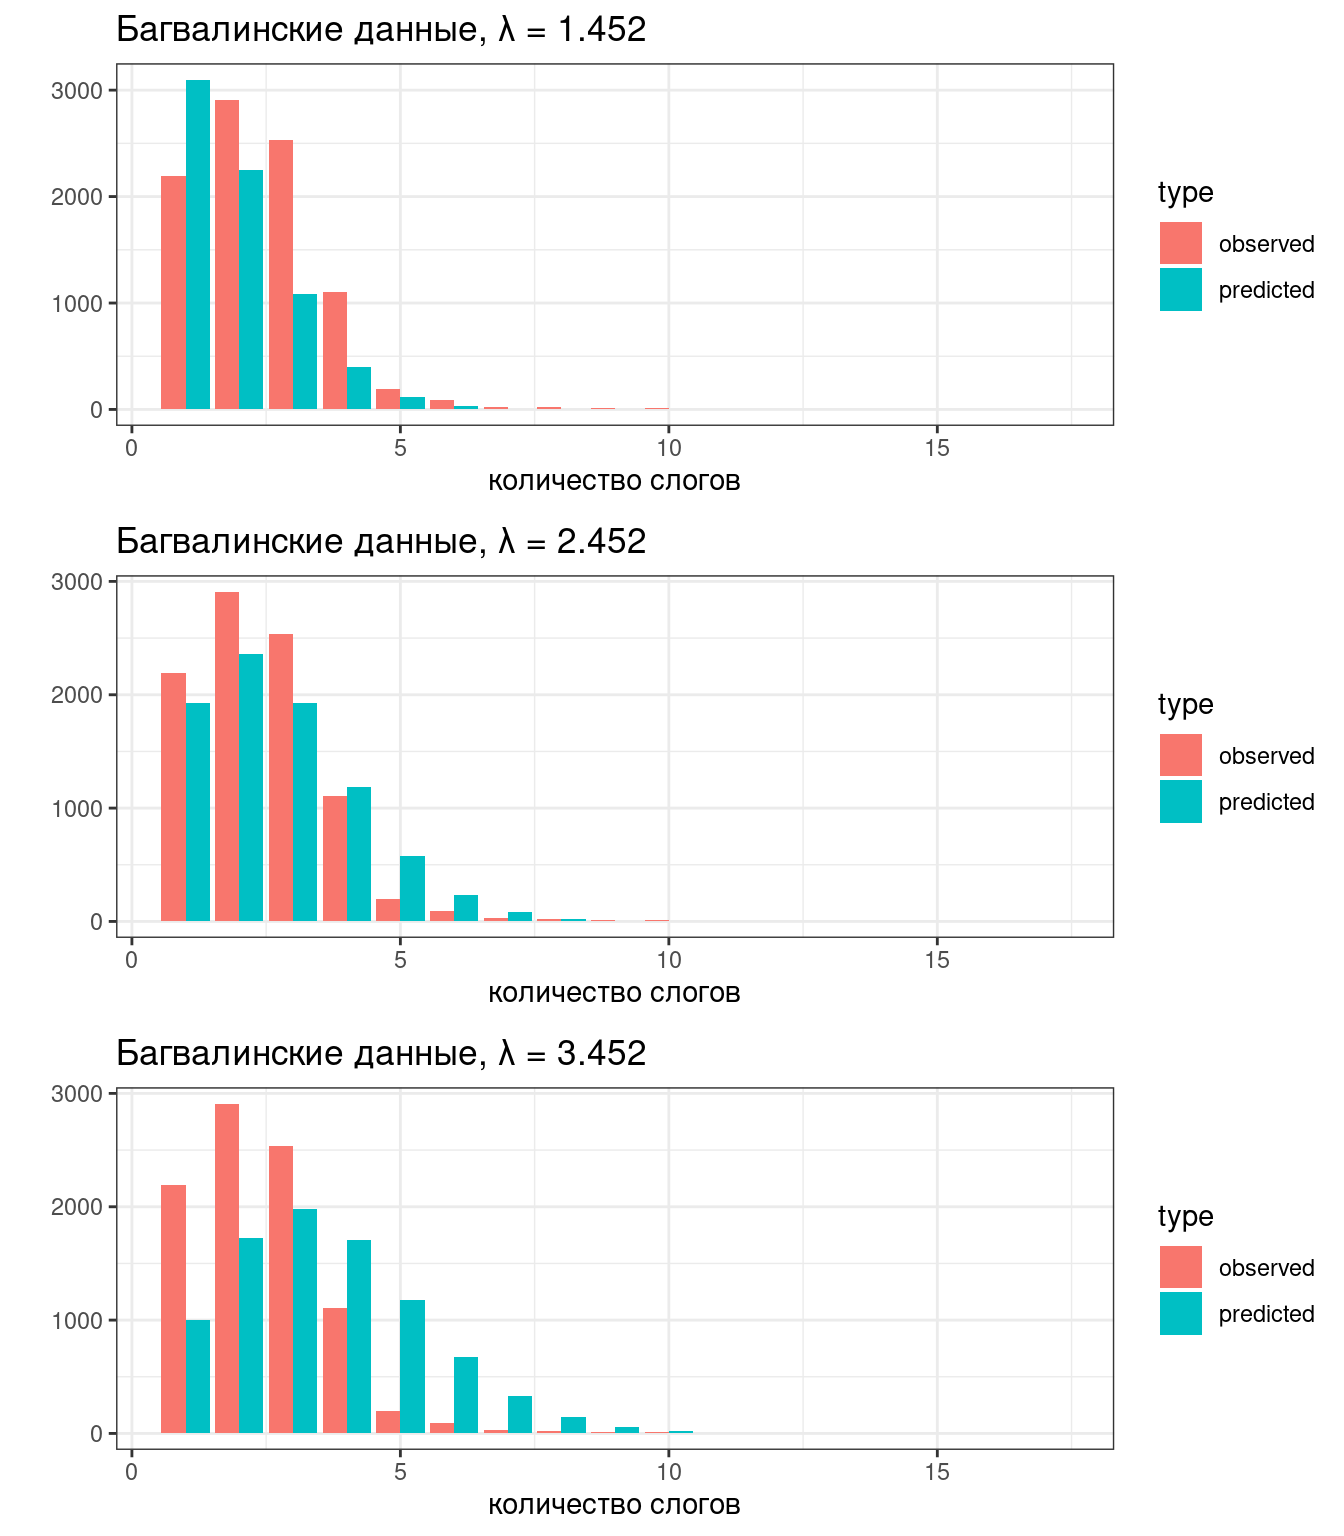
\includegraphics{da4l_files/figure-latex/unnamed-chunk-23-1.pdf}

\begin{rmdtask}
Выше было написано:

\begin{quote}
Согласно модели Пуассона все слова \textbf{независимо друг от друга}
получают сколько-то слогов согласно распределению Пуассона.
\end{quote}

Какие проблемы есть у предположения о независимости друг от друга
количества слогов разных слов в словаре?
\end{rmdtask}

\hypertarget{ux447ux438ux441ux43bux43eux432ux44bux435-ux43fux435ux440ux435ux43cux435ux43dux43dux44bux435}{%
\section{Числовые переменные}\label{ux447ux438ux441ux43bux43eux432ux44bux435-ux43fux435ux440ux435ux43cux435ux43dux43dux44bux435}}

\hypertarget{ux43dux43eux440ux43cux430ux43bux44cux43dux43eux435-ux440ux430ux441ux43fux440ux435ux434ux435ux43bux435ux43dux438ux435}{%
\subsection{Нормальное распределение}\label{ux43dux43eux440ux43cux430ux43bux44cux43dux43eux435-ux440ux430ux441ux43fux440ux435ux434ux435ux43bux435ux43dux438ux435}}

\[P(x) = \frac{1}{\sigma\sqrt{2\pi}}\times e^{-\frac{\left(x-\mu\right)^2}{2\sigma^2}}\]

\[\mu \in \mathbb{R}; \sigma^2 > 0\]

\begin{Shaded}
\begin{Highlighting}[]
\FunctionTok{tibble}\NormalTok{(}\AttributeTok{x =} \DecValTok{1}\SpecialCharTok{:}\DecValTok{100}\NormalTok{,}
       \AttributeTok{PDF =} \FunctionTok{dnorm}\NormalTok{(}\AttributeTok{x =}\NormalTok{ x, }\AttributeTok{mean =} \DecValTok{50}\NormalTok{, }\AttributeTok{sd =} \DecValTok{10}\NormalTok{)) }\SpecialCharTok{\%\textgreater{}\%} 
  \FunctionTok{ggplot}\NormalTok{(}\FunctionTok{aes}\NormalTok{(x, PDF))}\SpecialCharTok{+}
  \FunctionTok{geom\_point}\NormalTok{()}\SpecialCharTok{+}
  \FunctionTok{geom\_line}\NormalTok{()}\SpecialCharTok{+}
  \FunctionTok{labs}\NormalTok{(}\AttributeTok{title =} \StringTok{"PDF нормального распределения (μ = 50, sd = 10)"}\NormalTok{)}
\end{Highlighting}
\end{Shaded}

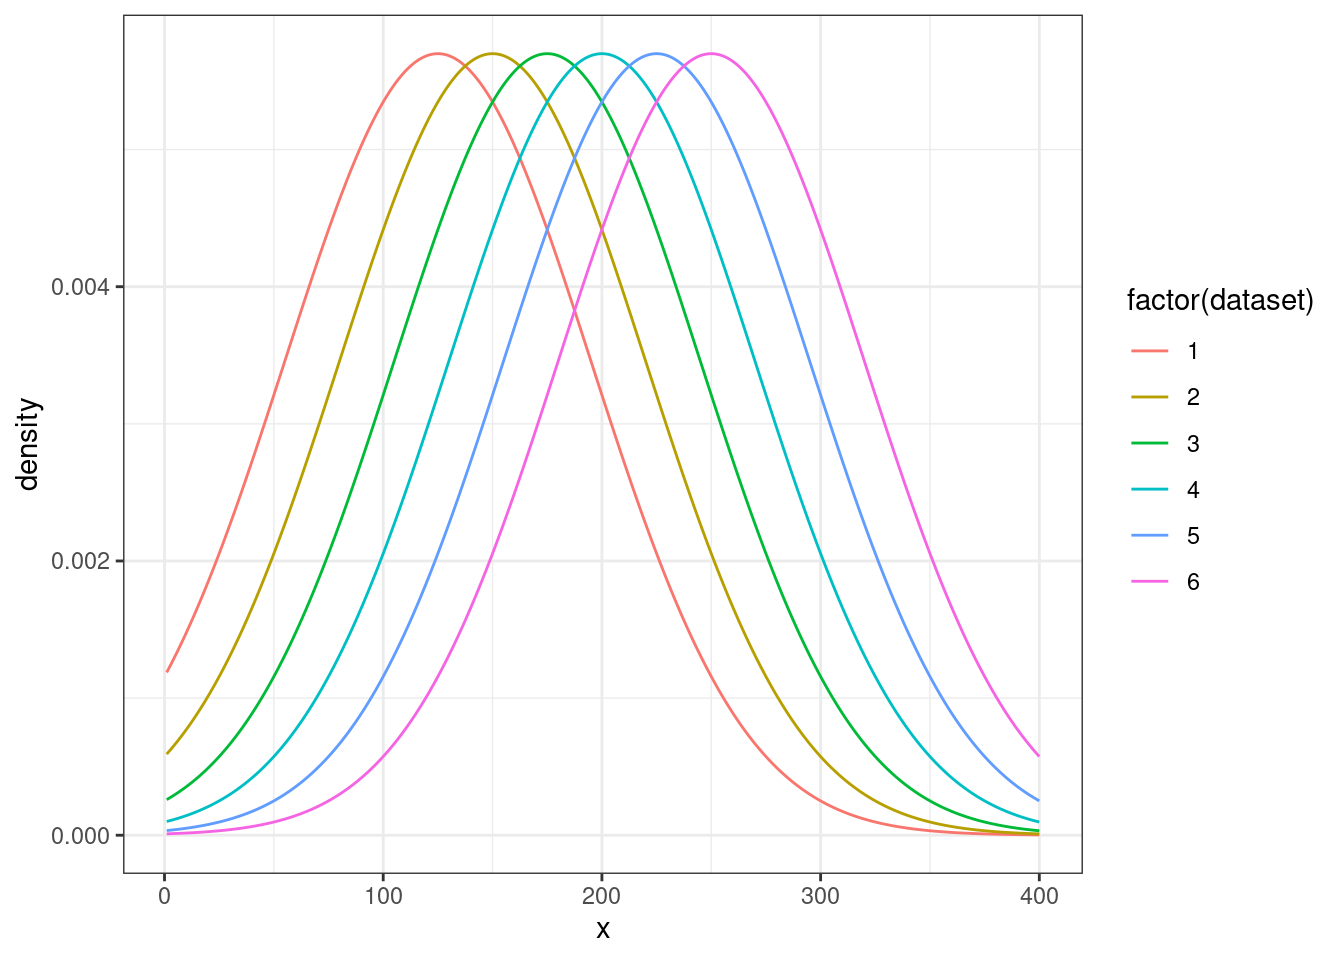
\includegraphics{da4l_files/figure-latex/unnamed-chunk-25-1.pdf}

Птичка напела, что длительность гласных американского английского из \citep{hillenbrand95} можно описать нормальным распределением с параметрами \(\mu =\) 274.673 и \(\sigma =\) 64.482. Посмотрим, как можно совместить данные и это распределение:

\begin{Shaded}
\begin{Highlighting}[]
\NormalTok{vowels }\OtherTok{\textless{}{-}} \FunctionTok{read\_csv}\NormalTok{(}\StringTok{"https://raw.githubusercontent.com/agricolamz/2021\_da4l/master/data/phonTools\_hillenbrand\_1995.csv"}\NormalTok{) }
\NormalTok{vowels }\SpecialCharTok{\%\textgreater{}\%} 
  \FunctionTok{ggplot}\NormalTok{(}\FunctionTok{aes}\NormalTok{(dur)) }\SpecialCharTok{+} 
  \FunctionTok{geom\_histogram}\NormalTok{(}\FunctionTok{aes}\NormalTok{(}\AttributeTok{y =}\NormalTok{..density..)) }\SpecialCharTok{+} \CommentTok{\# обратите внимание на аргумент ..density..}
  \FunctionTok{stat\_function}\NormalTok{(}\AttributeTok{fun =}\NormalTok{ dnorm, }\AttributeTok{args =} \FunctionTok{list}\NormalTok{(}\AttributeTok{mean =} \FloatTok{274.673}\NormalTok{, }\AttributeTok{sd =} \FloatTok{64.482}\NormalTok{), }\AttributeTok{color =} \StringTok{"red"}\NormalTok{)}
\end{Highlighting}
\end{Shaded}

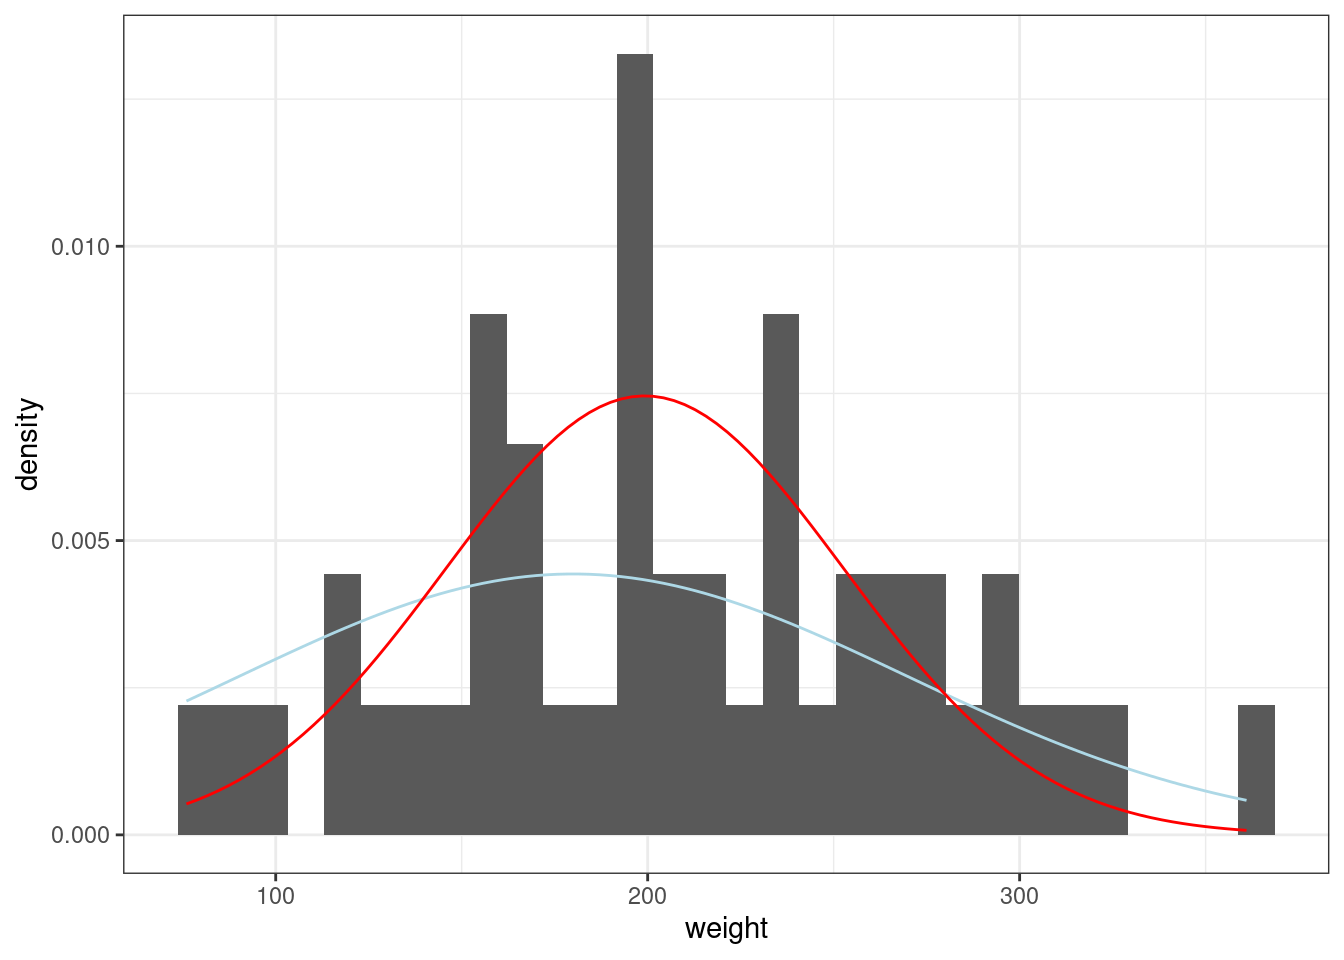
\includegraphics{da4l_files/figure-latex/unnamed-chunk-27-1.pdf}

\hypertarget{ux43bux43eux433ux43dux43eux440ux43cux430ux43bux44cux43dux43eux435-ux440ux430ux441ux43fux440ux435ux434ux435ux43bux435ux43dux438ux435}{%
\subsection{Логнормальное распределение}\label{ux43bux43eux433ux43dux43eux440ux43cux430ux43bux44cux43dux43eux435-ux440ux430ux441ux43fux440ux435ux434ux435ux43bux435ux43dux438ux435}}

\[P(x) = \frac{1}{\sqrt{x\sigma2\pi}}\times e^{-\frac{\left(\ln(x)-\mu\right)^2}{2\sigma^2}}\]

\[\mu \in \mathbb{R}; \sigma^2 > 0\]

\begin{Shaded}
\begin{Highlighting}[]
\FunctionTok{tibble}\NormalTok{(}\AttributeTok{x =} \DecValTok{1}\SpecialCharTok{:}\DecValTok{100}\NormalTok{,}
       \AttributeTok{PDF =} \FunctionTok{dlnorm}\NormalTok{(}\AttributeTok{x =}\NormalTok{ x, }\AttributeTok{mean =} \DecValTok{3}\NormalTok{, }\AttributeTok{sd =} \FloatTok{0.5}\NormalTok{)) }\SpecialCharTok{\%\textgreater{}\%} 
  \FunctionTok{ggplot}\NormalTok{(}\FunctionTok{aes}\NormalTok{(x, PDF))}\SpecialCharTok{+}
  \FunctionTok{geom\_point}\NormalTok{()}\SpecialCharTok{+}
  \FunctionTok{geom\_line}\NormalTok{()}\SpecialCharTok{+}
  \FunctionTok{labs}\NormalTok{(}\AttributeTok{title =} \StringTok{"PDF логнормального распределения (μ = 3, σ = 0.5)"}\NormalTok{)}
\end{Highlighting}
\end{Shaded}

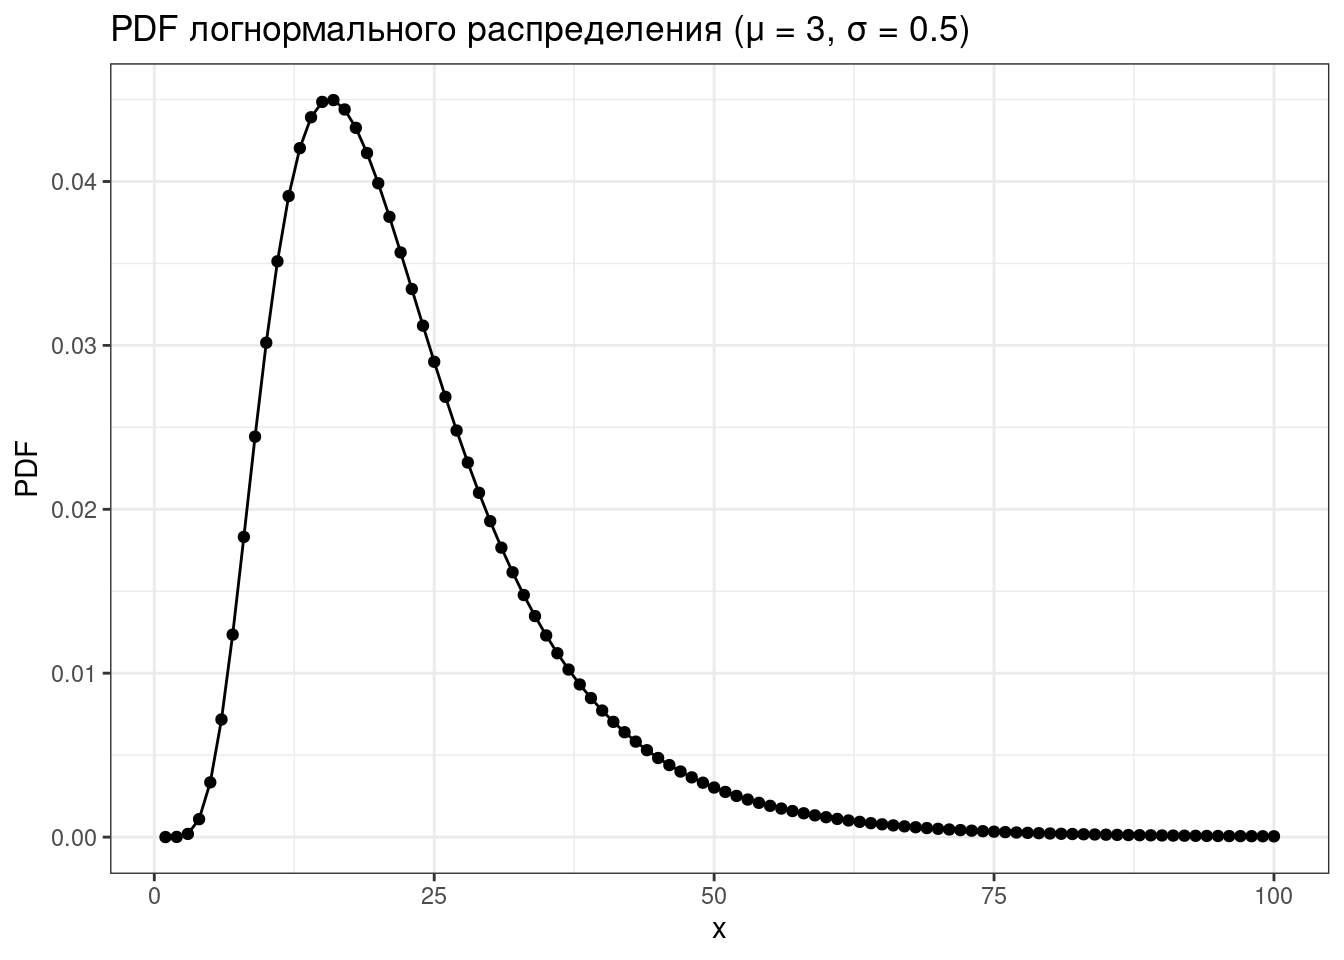
\includegraphics{da4l_files/figure-latex/unnamed-chunk-28-1.pdf}

\begin{rmdtask}
Какая из логнормальных моделей для длительности гласных американского
английского из {[}@hillenbrand95{]} лучше подходит к данным? Попробуйте
самостоятельно построить данный график.
\end{rmdtask}

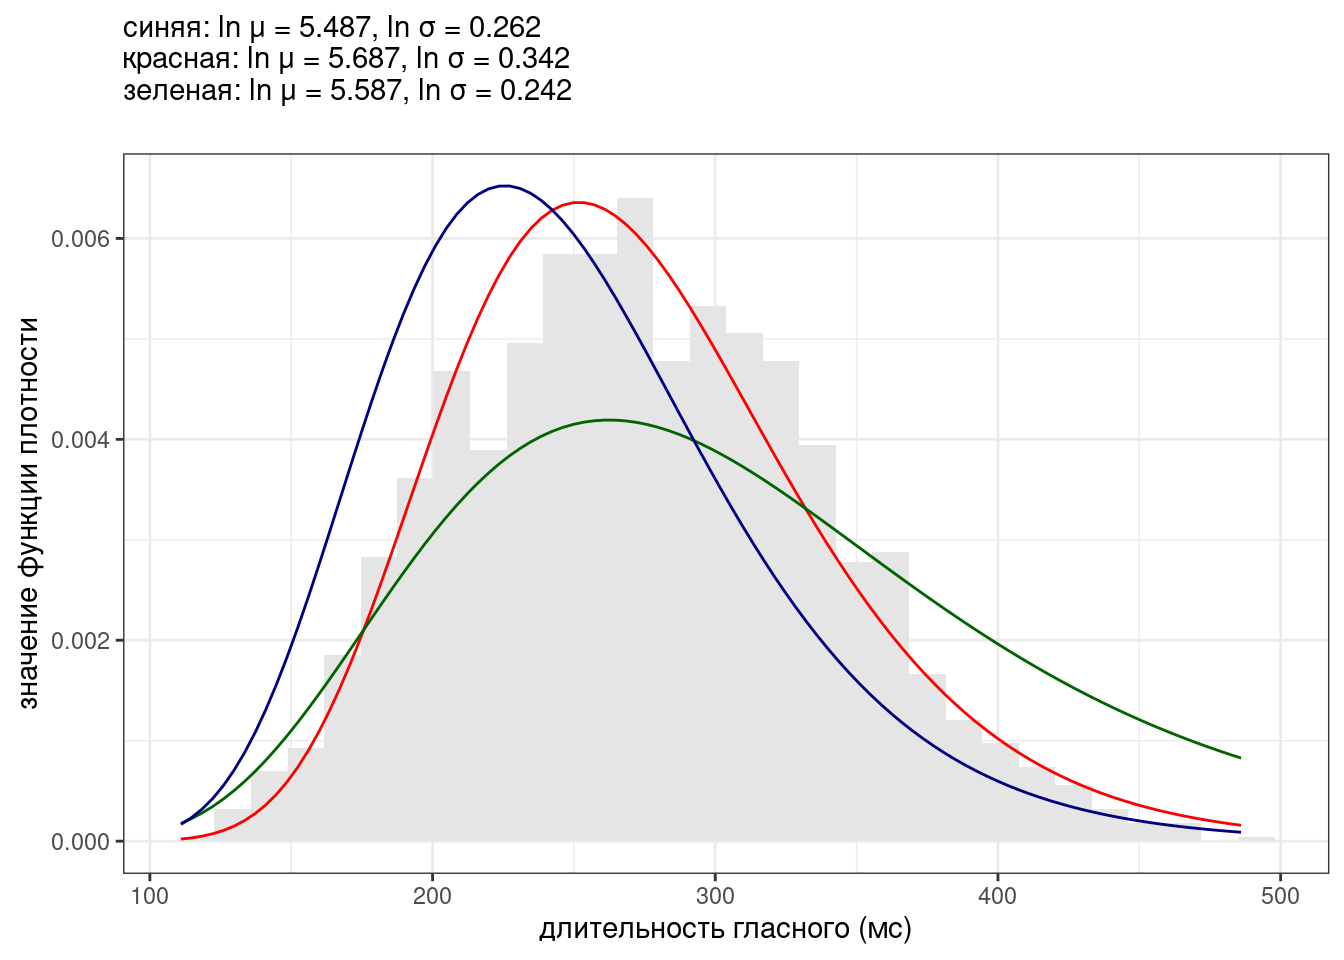
\includegraphics{da4l_files/figure-latex/unnamed-chunk-31-1.pdf}

\hypertarget{ux447ux442ux43e-ux435ux449ux435-ux43fux43eux447ux438ux442ux430ux442ux44c-ux43fux440ux43e-ux440ux430ux441ux43fux440ux435ux434ux435ux43bux435ux43dux438ux44f}{%
\subsection{Что еще почитать про распределения?}\label{ux447ux442ux43e-ux435ux449ux435-ux43fux43eux447ux438ux442ux430ux442ux44c-ux43fux440ux43e-ux440ux430ux441ux43fux440ux435ux434ux435ux43bux435ux43dux438ux44f}}

Люди придумали очень много разных распределений. Стоит, наверное, также понимать, что распределения не существуют отдельно в вакууме: многие из них математически связаны друг с другом. Про это можно посмотреть \href{http://www.math.wm.edu/~leemis/chart/UDR/UDR.html}{вот здесь} или \href{https://en.wikipedia.org/wiki/Relationships_among_probability_distributions}{здесь}.

\hypertarget{ux43cux435ux442ux43eux434-ux43cux430ux43aux441ux438ux43cux430ux43bux44cux43dux43eux433ux43e-ux43fux440ux430ux432ux434ux43eux43fux43eux434ux43eux431ux438ux44f}{%
\chapter{Метод максимального правдоподобия}\label{ux43cux435ux442ux43eux434-ux43cux430ux43aux441ux438ux43cux430ux43bux44cux43dux43eux433ux43e-ux43fux440ux430ux432ux434ux43eux43fux43eux434ux43eux431ux438ux44f}}

\hypertarget{ux43eux446ux435ux43dux43aux430-ux432ux435ux440ux43eux44fux442ux43dux43eux441ux442ux438}{%
\section{Оценка вероятности}\label{ux43eux446ux435ux43dux43aux430-ux432ux435ux440ux43eux44fux442ux43dux43eux441ux442ux438}}

\begin{Shaded}
\begin{Highlighting}[]
\FunctionTok{library}\NormalTok{(tidyverse)}
\end{Highlighting}
\end{Shaded}

Когда у нас задано некоторое распределение, мы можем задавать к нему разные вопросы. Например, если мы верим что длительность гласных американского английского из \citep{hillenbrand95} можно описать логнормальным распределением с параметрами \(\ln{\mu} =\) 5.587 и \(\ln{\sigma} =\) 0.242, то мы можем делать некотрые предсказания относительно интересующей нас переменной.

\begin{Shaded}
\begin{Highlighting}[]
\FunctionTok{ggplot}\NormalTok{() }\SpecialCharTok{+} 
  \FunctionTok{stat\_function}\NormalTok{(}\AttributeTok{fun =}\NormalTok{ dlnorm, }\AttributeTok{args =} \FunctionTok{list}\NormalTok{(}\AttributeTok{mean =} \FloatTok{5.587}\NormalTok{, }\AttributeTok{sd =} \FloatTok{0.242}\NormalTok{))}\SpecialCharTok{+}
  \FunctionTok{scale\_x\_continuous}\NormalTok{(}\AttributeTok{breaks =} \DecValTok{0}\SpecialCharTok{:}\DecValTok{6}\SpecialCharTok{*}\DecValTok{100}\NormalTok{, }\AttributeTok{limits =} \FunctionTok{c}\NormalTok{(}\DecValTok{0}\NormalTok{, }\DecValTok{650}\NormalTok{))}\SpecialCharTok{+}
  \FunctionTok{labs}\NormalTok{(}\AttributeTok{x =} \StringTok{"длительность гласного (мс)"}\NormalTok{,}
       \AttributeTok{y =} \StringTok{"значение функции плотности"}\NormalTok{)}
\end{Highlighting}
\end{Shaded}

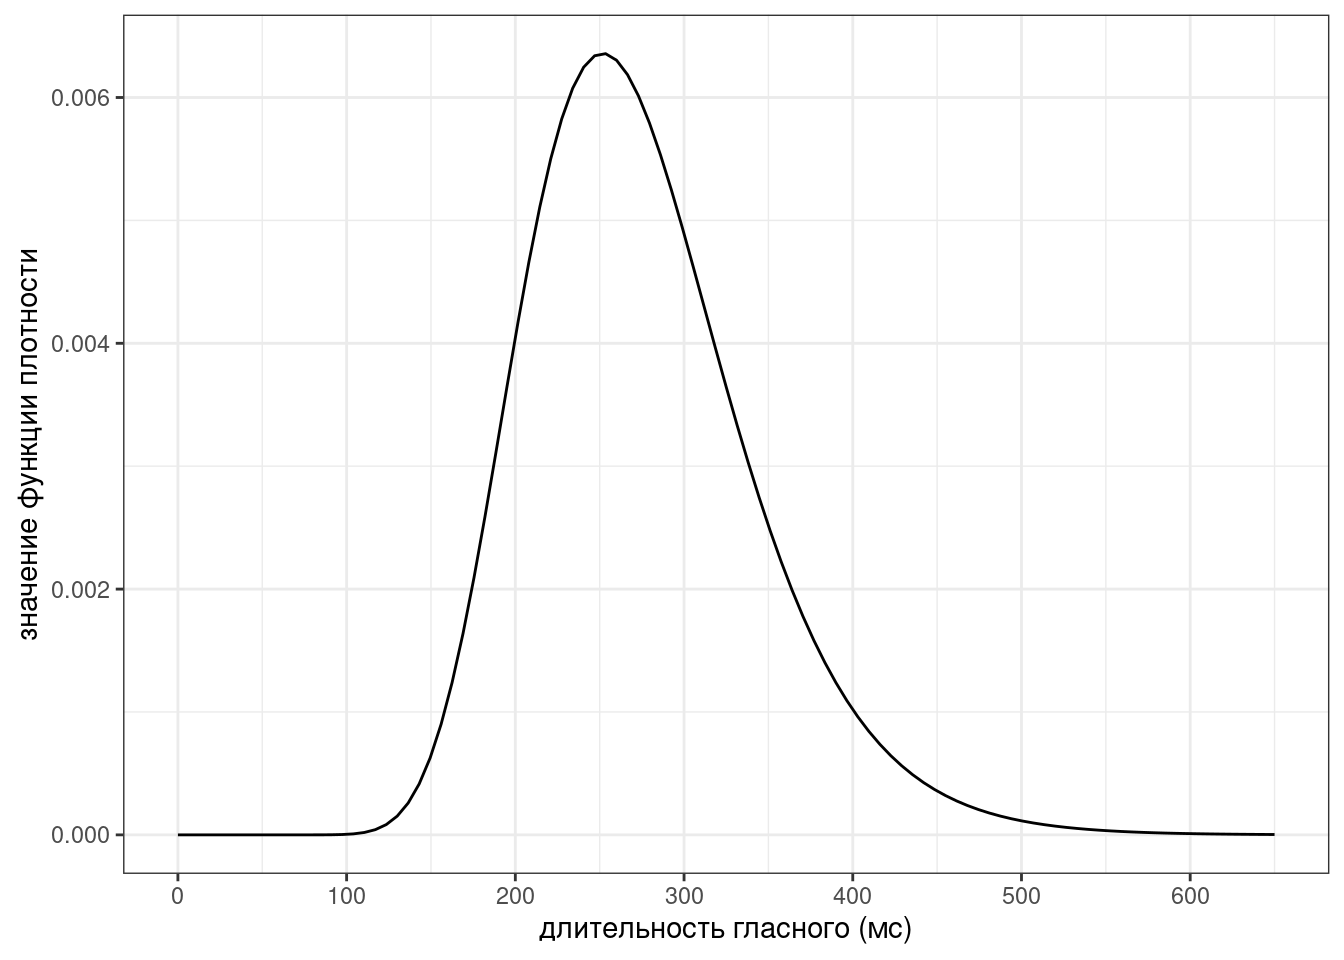
\includegraphics{da4l_files/figure-latex/unnamed-chunk-34-1.pdf}

\begin{rmdtask}
Если принять на веру, что логнормальное распределение с параметрами
\(\ln{\mu} =\) 5.587 и \(\ln{\sigma}=\) 0.242 описывает данные
длительности гласных американского английского из {[}@hillenbrand95{]},
то какова вероятность наблюдать значения между 300 и 400 мс? То же самое
можно записать, используя математическую нотацию:

\[P\left(X \in [300,\, 400] | X \sim \ln{\mathcal{N}}(\ln{\mu} = 5.587, \ln{\sigma}=0.242)\right) = ??\]
Ответ округлите до трех и меньше знаков после запятой.
\end{rmdtask}

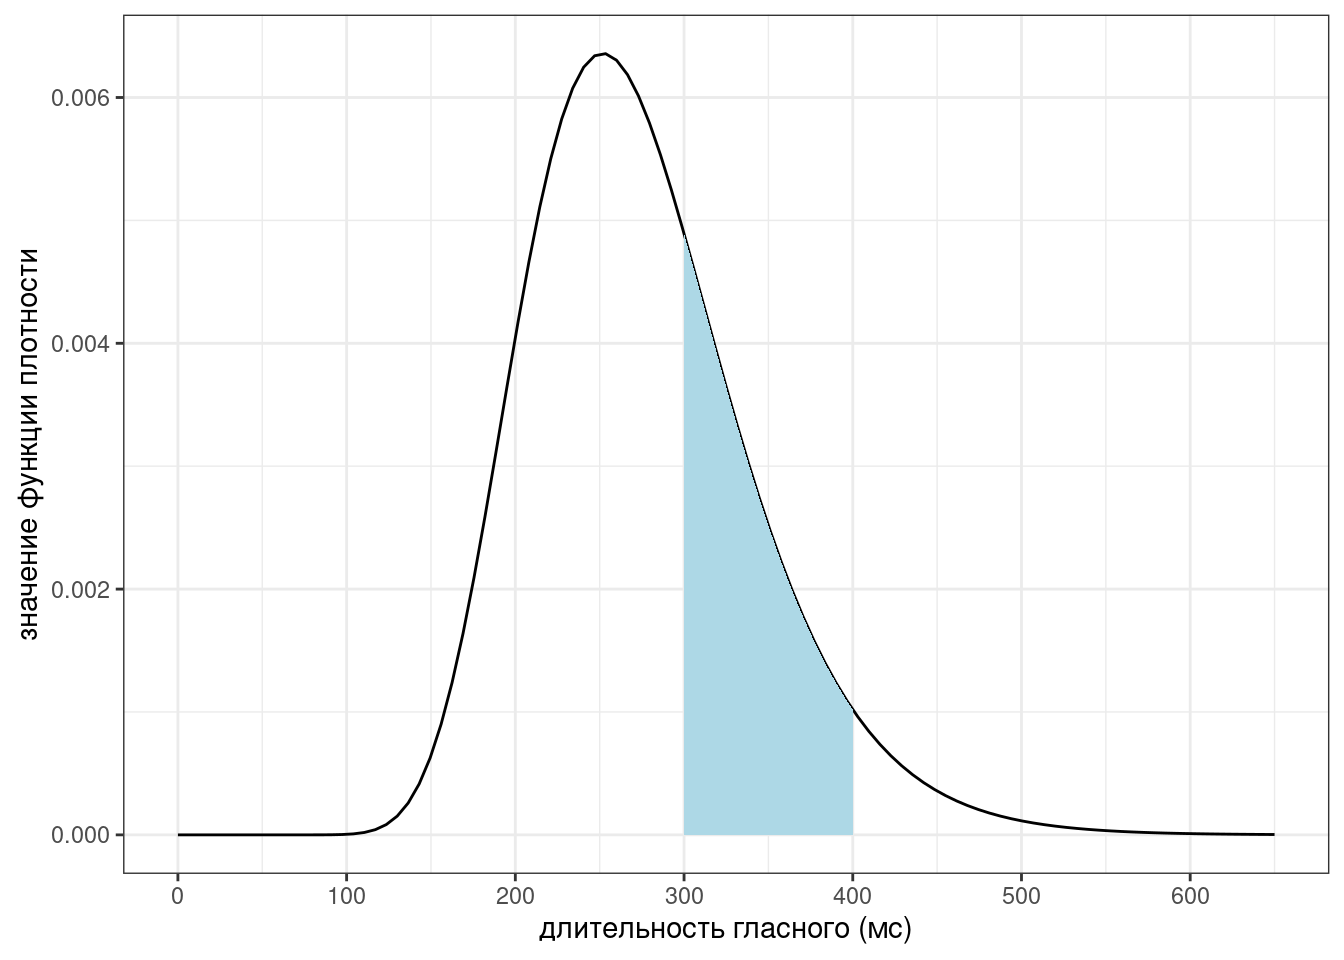
\includegraphics{da4l_files/figure-latex/unnamed-chunk-36-1.pdf}

\begin{rmdtask}
Если принять на веру, что биномиальное распределение с параметрами
\(p =\) 0.9 описывает, согласно {[}@rosenbach03: 394{]} употребление
\emph{s}-генитивов в британском английском, то какова вероятность
наблюдать значения между 300 и 350 генитивов в интервью, содержащее 400
генитивных контекстов? То же самое можно записать, используя
математическую нотацию:

\[P\left(X \in [300,\, 350] | X \sim Binom(n = 400, p = 0.9)\right) = ??\]
Ответ округлите до трех и меньше знаков после запятой.
\end{rmdtask}

\hypertarget{ux444ux443ux43dux43aux446ux438ux44f-ux43fux440ux430ux432ux434ux43eux43fux43eux434ux43eux431ux438ux44f}{%
\section{Функция правдоподобия}\label{ux444ux443ux43dux43aux446ux438ux44f-ux43fux440ux430ux432ux434ux43eux43fux43eux434ux43eux431ux438ux44f}}

Если при поиске вероятностей, мы предполагали, что данные нам \textbf{неизвестны}, а распределение и его параметры \textbf{известны}, то функция правдоподобия позволяет этот процесс перевернуть, запустив поиск параметров распределения, при изветсных данных и семье распределения:

\[L\left(X \sim Distr(...)|x\right) = ...\]

Таким образом получается, что на основании функции плотности мы можем сравнивать, какой параметр лучше подходит к нашим данным.

Для примера рассмотрим наш s-генетив: мы провели интервью и нам встретилось 85 \emph{s}-генетивов из 100 случаев всех генетивов. Насколько хорошо подходит нам распределение с параметром \emph{p} = 0.9?

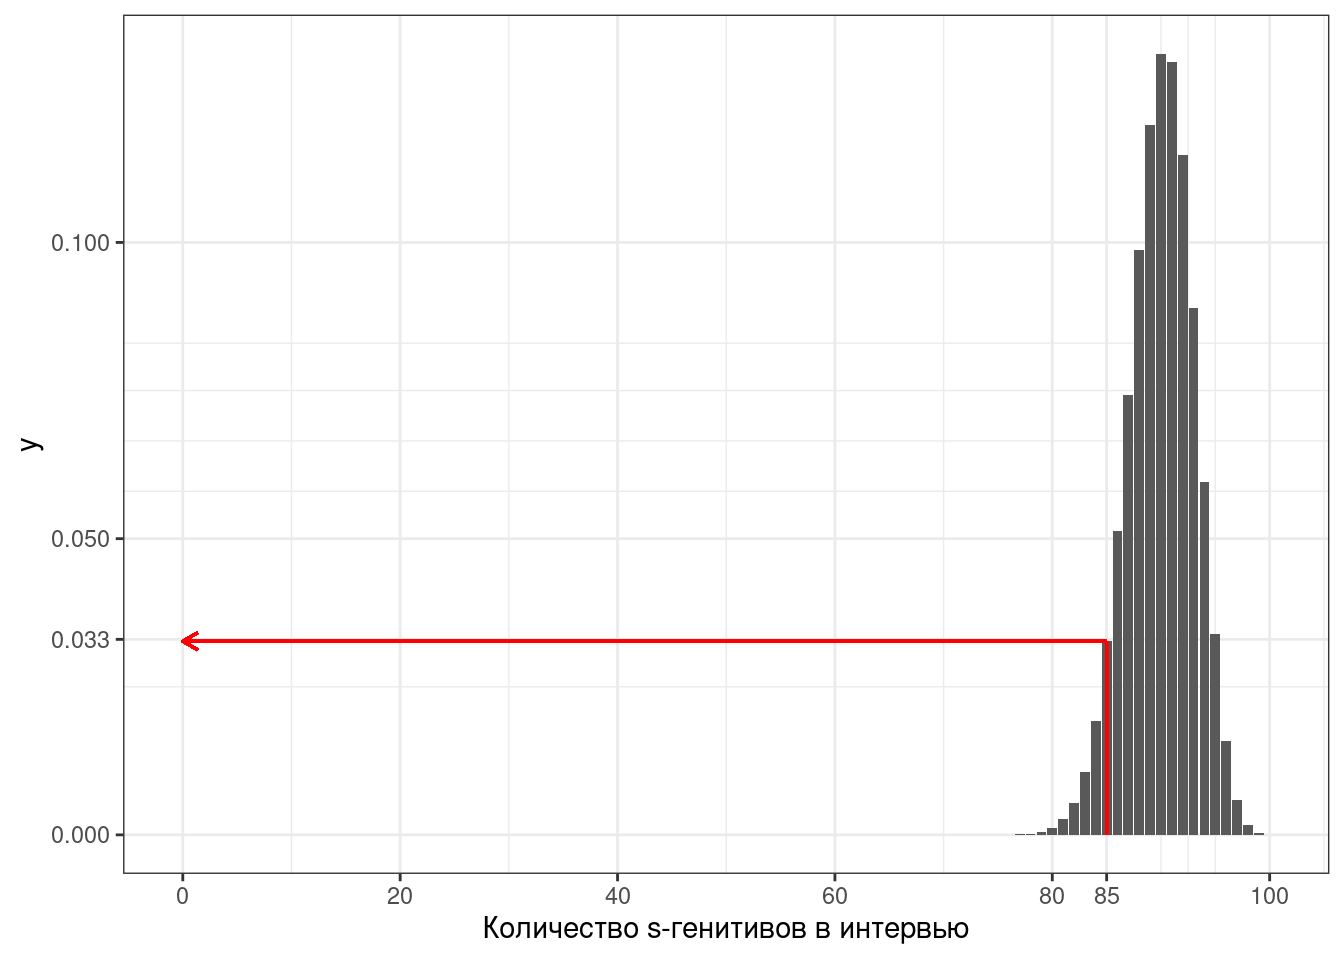
\includegraphics{da4l_files/figure-latex/unnamed-chunk-40-1.pdf}

Ответ:

\begin{Shaded}
\begin{Highlighting}[]
\FunctionTok{dbinom}\NormalTok{(}\DecValTok{85}\NormalTok{, }\DecValTok{100}\NormalTok{, }\FloatTok{0.9}\NormalTok{)}
\end{Highlighting}
\end{Shaded}

\begin{verbatim}
[1] 0.03268244
\end{verbatim}

Представим теперь это как функцию от параметра \emph{p}:

\begin{Shaded}
\begin{Highlighting}[]
\FunctionTok{tibble}\NormalTok{(}\AttributeTok{p =} \FunctionTok{seq}\NormalTok{(}\DecValTok{0}\NormalTok{, }\DecValTok{1}\NormalTok{, }\AttributeTok{by =} \FloatTok{0.01}\NormalTok{)) }\SpecialCharTok{\%\textgreater{}\%} 
  \FunctionTok{ggplot}\NormalTok{(}\FunctionTok{aes}\NormalTok{(p)) }\SpecialCharTok{+}
  \FunctionTok{stat\_function}\NormalTok{(}\AttributeTok{fun =} \ControlFlowTok{function}\NormalTok{(p) }\FunctionTok{dbinom}\NormalTok{(}\DecValTok{85}\NormalTok{, }\DecValTok{100}\NormalTok{, p), }\AttributeTok{geom =} \StringTok{"col"}\NormalTok{)}\SpecialCharTok{+}
  \FunctionTok{labs}\NormalTok{(}\AttributeTok{x =} \StringTok{"параметр биномиального распределения p"}\NormalTok{,}
       \AttributeTok{y =} \StringTok{"значение функции правдоподобия}\SpecialCharTok{\textbackslash{}n}\StringTok{(одно наблюдение)"}\NormalTok{)}
\end{Highlighting}
\end{Shaded}

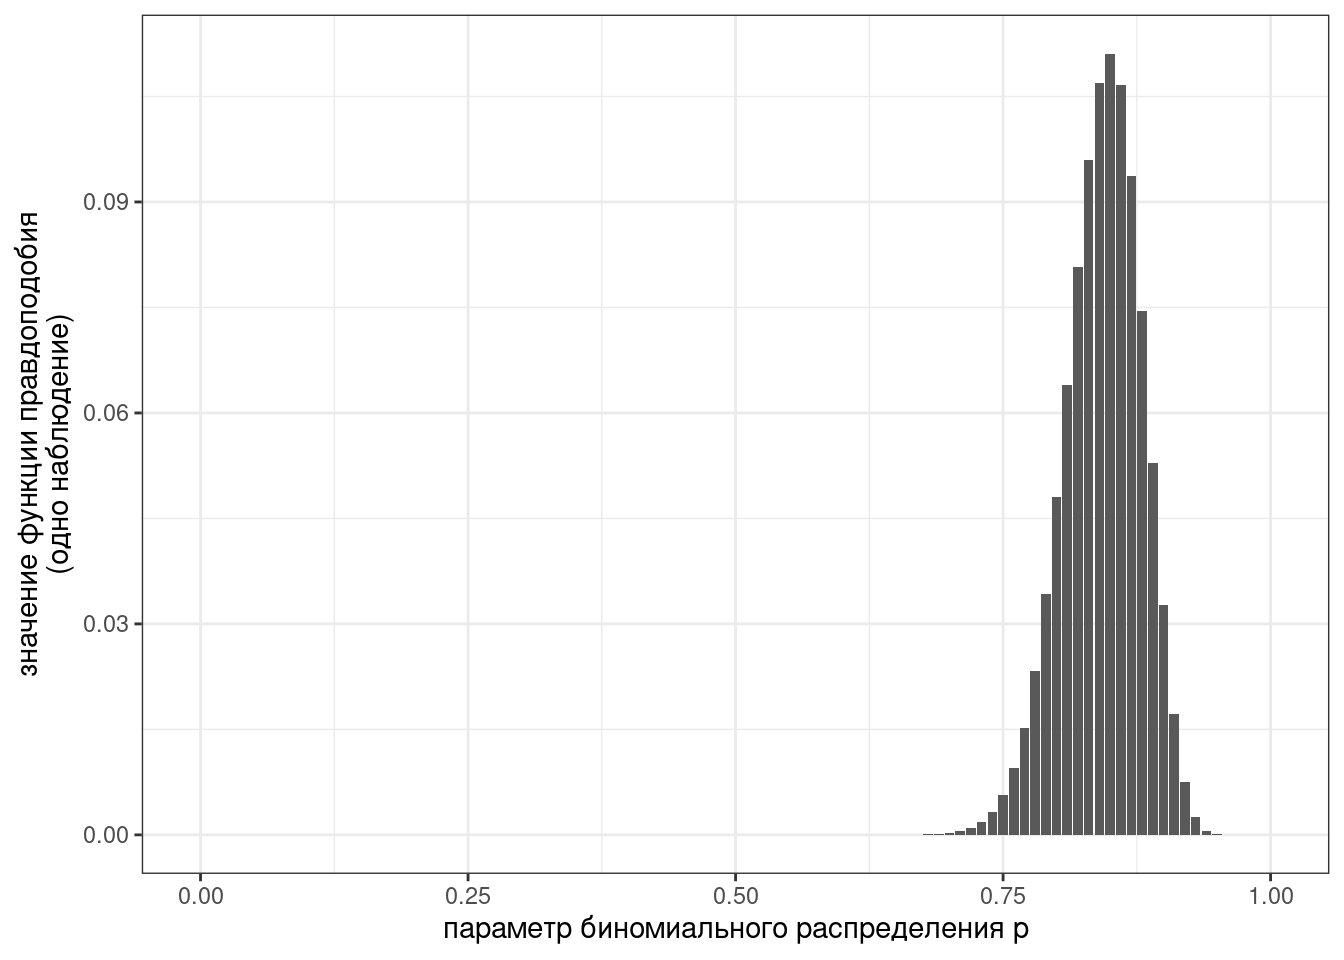
\includegraphics{da4l_files/figure-latex/unnamed-chunk-42-1.pdf}

А что если мы располагаем двумя интервью одного актера? В первом на сто генитивов пришлось 85 s-генитивов, а во втором -- 89. В таком случае, также как и с вероятностью наступления двух независимых событий, значения функции плотности перемножаются.

\begin{Shaded}
\begin{Highlighting}[]
\FunctionTok{dbinom}\NormalTok{(}\DecValTok{85}\NormalTok{, }\DecValTok{100}\NormalTok{, }\FloatTok{0.9}\NormalTok{)}\SpecialCharTok{*}\FunctionTok{dbinom}\NormalTok{(}\DecValTok{89}\NormalTok{, }\DecValTok{100}\NormalTok{, }\FloatTok{0.9}\NormalTok{)}
\end{Highlighting}
\end{Shaded}

\begin{verbatim}
[1] 0.003917892
\end{verbatim}

\begin{Shaded}
\begin{Highlighting}[]
\FunctionTok{tibble}\NormalTok{(}\AttributeTok{p =} \FunctionTok{seq}\NormalTok{(}\DecValTok{0}\NormalTok{, }\DecValTok{1}\NormalTok{, }\AttributeTok{by =} \FloatTok{0.01}\NormalTok{)) }\SpecialCharTok{\%\textgreater{}\%} 
  \FunctionTok{ggplot}\NormalTok{(}\FunctionTok{aes}\NormalTok{(p)) }\SpecialCharTok{+}
  \FunctionTok{stat\_function}\NormalTok{(}\AttributeTok{fun =} \ControlFlowTok{function}\NormalTok{(p) }\FunctionTok{dbinom}\NormalTok{(}\DecValTok{85}\NormalTok{, }\DecValTok{100}\NormalTok{, p)}\SpecialCharTok{*}\FunctionTok{dbinom}\NormalTok{(}\DecValTok{89}\NormalTok{, }\DecValTok{100}\NormalTok{, p), }\AttributeTok{geom =} \StringTok{"col"}\NormalTok{)}\SpecialCharTok{+}
  \FunctionTok{labs}\NormalTok{(}\AttributeTok{x =} \StringTok{"параметр биномиального распределения p"}\NormalTok{,}
       \AttributeTok{y =} \StringTok{"значение функции правдоподобия}\SpecialCharTok{\textbackslash{}n}\StringTok{(два наблюдения)"}\NormalTok{)}
\end{Highlighting}
\end{Shaded}

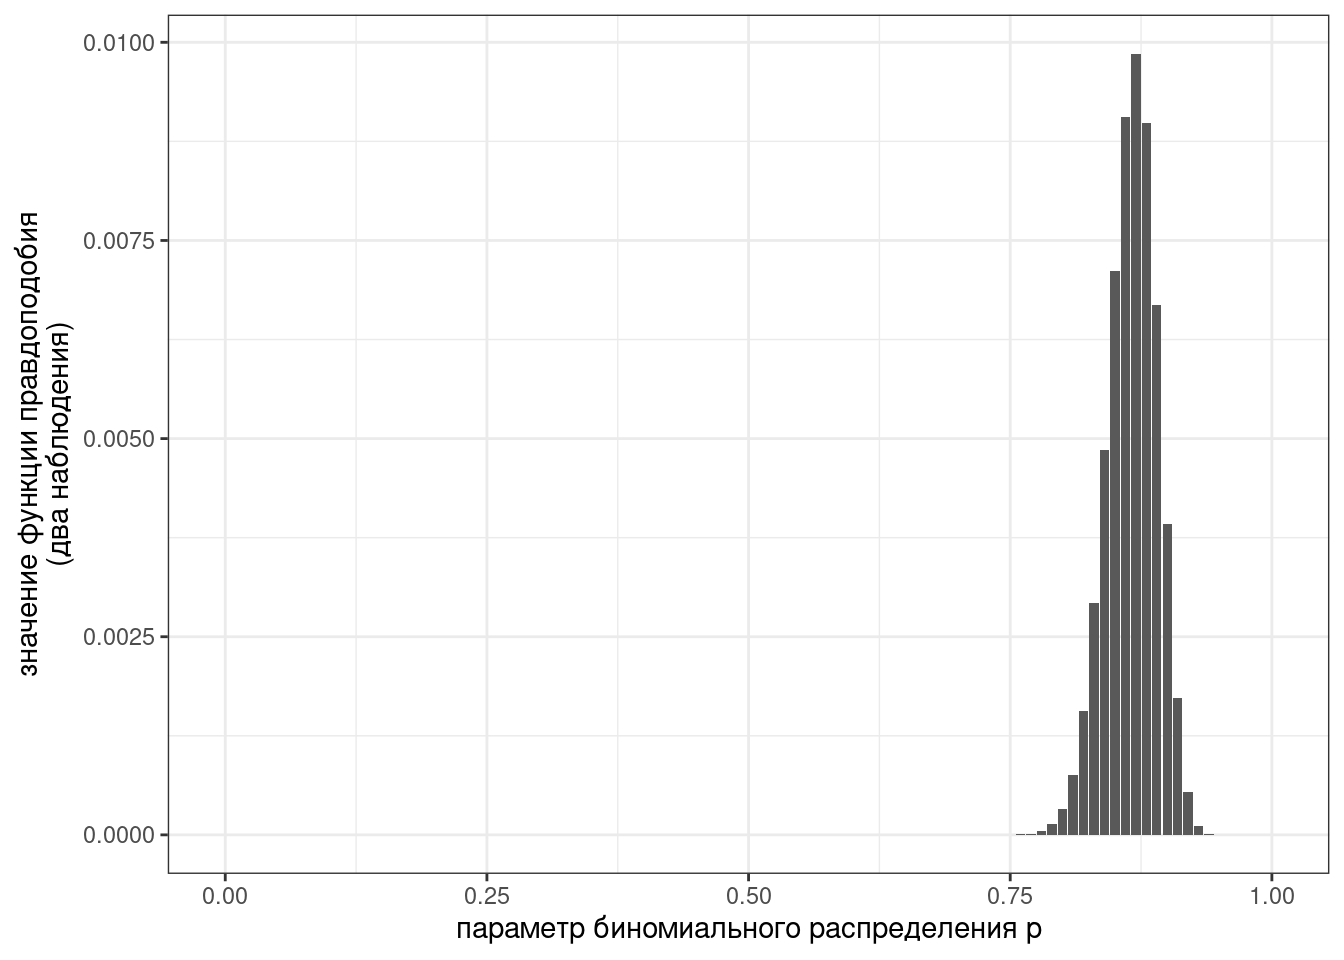
\includegraphics{da4l_files/figure-latex/unnamed-chunk-44-1.pdf}

В итоге:

\begin{itemize}
\tightlist
\item
  вероятность --- P(data\textbar distribution)
\item
  правдоподобие --- L(distribution\textbar data)
\end{itemize}

Интеграл распределения/сумма значений вероятностей равен/на 1. \href{https://stats.stackexchange.com/a/31241/225843}{Интеграл распределения/сумма значений правдоподобия может быть не равен/на 1}.

\hypertarget{ux43fux440ux438ux43cux435ux440-ux441-ux43dux435ux43fux440ux435ux440ux44bux432ux43dux44bux43c-ux440ux430ux441ux43fux440ux435ux434ux435ux43bux435ux43dux438ux435ux43c}{%
\section{Пример с непрерывным распределением}\label{ux43fux440ux438ux43cux435ux440-ux441-ux43dux435ux43fux440ux435ux440ux44bux432ux43dux44bux43c-ux440ux430ux441ux43fux440ux435ux434ux435ux43bux435ux43dux438ux435ux43c}}

Мы уже обсуждали, что длительность гласных американского английского из \citep{hillenbrand95} можно описать логнормальным распределением с параметрами \(\ln\mu\) и \(\ln\sigma\). Предположим, что \(\ln\sigma = 0.342\), построим функцию правдоподобия для \(\ln\mu\):

\begin{Shaded}
\begin{Highlighting}[]
\NormalTok{vowels }\OtherTok{\textless{}{-}} \FunctionTok{read\_csv}\NormalTok{(}\StringTok{"https://raw.githubusercontent.com/agricolamz/2022\_da4l/master/data/phonTools\_hillenbrand\_1995.csv"}\NormalTok{) }

\FunctionTok{tibble}\NormalTok{(}\AttributeTok{ln\_mu =} \FunctionTok{seq}\NormalTok{(}\DecValTok{5}\NormalTok{, }\DecValTok{6}\NormalTok{, }\AttributeTok{by =} \FloatTok{0.001}\NormalTok{)) }\SpecialCharTok{\%\textgreater{}\%} 
  \FunctionTok{ggplot}\NormalTok{(}\FunctionTok{aes}\NormalTok{(ln\_mu)) }\SpecialCharTok{+} 
  \FunctionTok{stat\_function}\NormalTok{(}\AttributeTok{fun =} \ControlFlowTok{function}\NormalTok{(ln\_mu) }\FunctionTok{dlnorm}\NormalTok{(vowels}\SpecialCharTok{$}\NormalTok{dur[}\DecValTok{1}\NormalTok{], }\AttributeTok{meanlog =}\NormalTok{ ln\_mu, }\AttributeTok{sdlog =} \FloatTok{0.242}\NormalTok{))}\SpecialCharTok{+}
  \FunctionTok{labs}\NormalTok{(}\AttributeTok{x =} \StringTok{"параметр логнормального распределения ln μ"}\NormalTok{,}
       \AttributeTok{y =} \StringTok{"значение функции правдоподобия}\SpecialCharTok{\textbackslash{}n}\StringTok{(одно наблюдение)"}\NormalTok{)}
\end{Highlighting}
\end{Shaded}

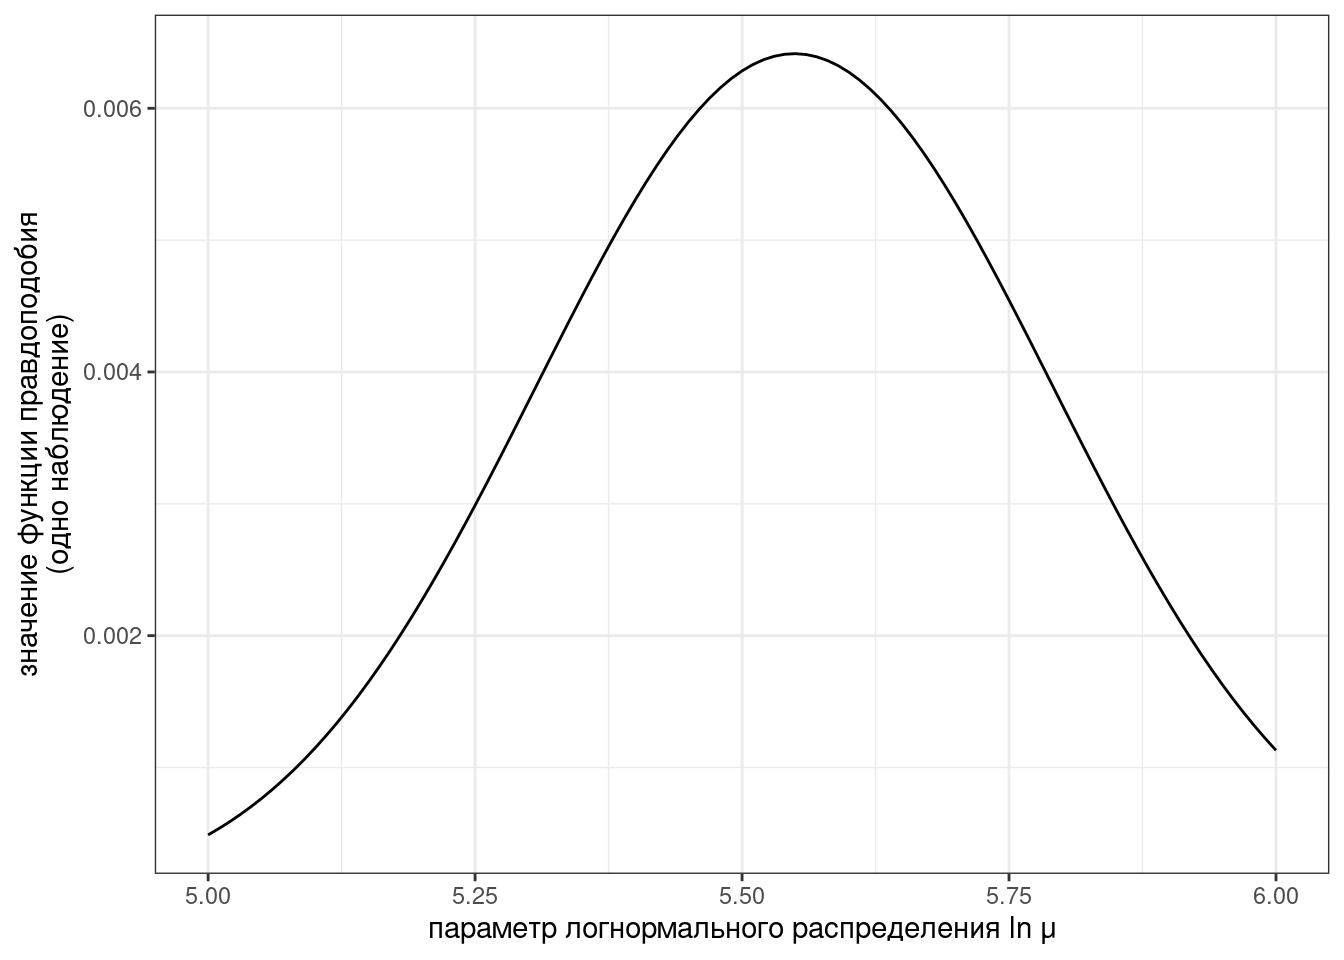
\includegraphics{da4l_files/figure-latex/unnamed-chunk-45-1.pdf}

\begin{Shaded}
\begin{Highlighting}[]
\FunctionTok{tibble}\NormalTok{(}\AttributeTok{ln\_mu =} \FunctionTok{seq}\NormalTok{(}\DecValTok{5}\NormalTok{, }\DecValTok{6}\NormalTok{, }\AttributeTok{by =} \FloatTok{0.001}\NormalTok{)) }\SpecialCharTok{\%\textgreater{}\%} 
  \FunctionTok{ggplot}\NormalTok{(}\FunctionTok{aes}\NormalTok{(ln\_mu)) }\SpecialCharTok{+} 
  \FunctionTok{stat\_function}\NormalTok{(}\AttributeTok{fun =} \ControlFlowTok{function}\NormalTok{(ln\_mu) }\FunctionTok{dlnorm}\NormalTok{(vowels}\SpecialCharTok{$}\NormalTok{dur[}\DecValTok{1}\NormalTok{], }\AttributeTok{meanlog =}\NormalTok{ ln\_mu, }\AttributeTok{sdlog =} \FloatTok{0.242}\NormalTok{)}\SpecialCharTok{*}\FunctionTok{dlnorm}\NormalTok{(vowels}\SpecialCharTok{$}\NormalTok{dur[}\DecValTok{2}\NormalTok{], }\AttributeTok{meanlog =}\NormalTok{ ln\_mu, }\AttributeTok{sdlog =} \FloatTok{0.242}\NormalTok{))}\SpecialCharTok{+}
  \FunctionTok{labs}\NormalTok{(}\AttributeTok{x =} \StringTok{"параметр логнормального распределения ln μ"}\NormalTok{,}
       \AttributeTok{y =} \StringTok{"значение функции правдоподобия}\SpecialCharTok{\textbackslash{}n}\StringTok{(два наблюдения)"}\NormalTok{)}
\end{Highlighting}
\end{Shaded}

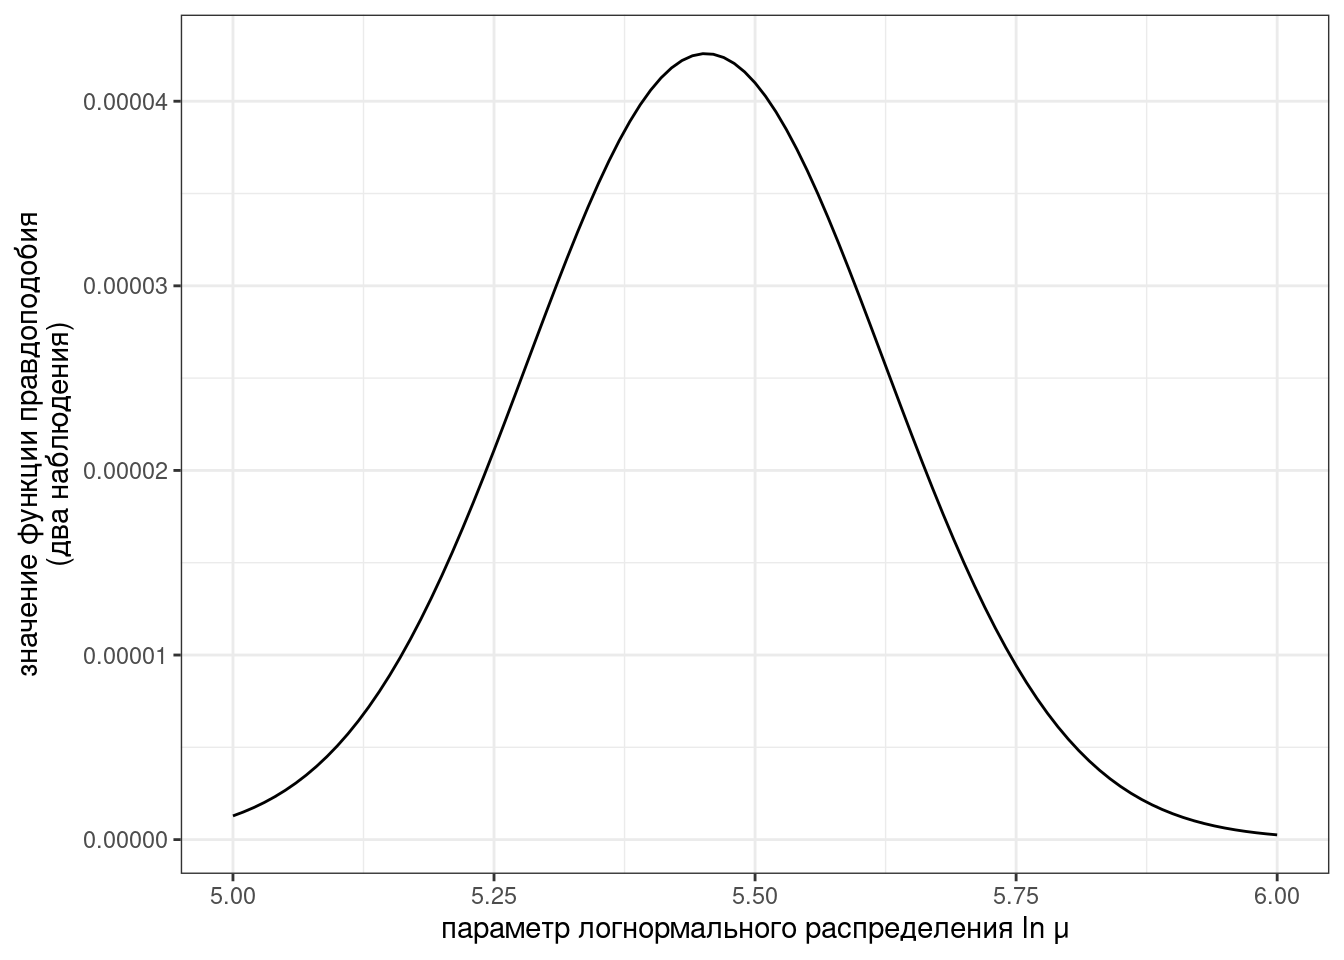
\includegraphics{da4l_files/figure-latex/unnamed-chunk-45-2.pdf}

\begin{Shaded}
\begin{Highlighting}[]
\FunctionTok{tibble}\NormalTok{(}\AttributeTok{ln\_mu =} \FunctionTok{seq}\NormalTok{(}\DecValTok{5}\NormalTok{, }\DecValTok{6}\NormalTok{, }\AttributeTok{by =} \FloatTok{0.001}\NormalTok{)) }\SpecialCharTok{\%\textgreater{}\%} 
  \FunctionTok{ggplot}\NormalTok{(}\FunctionTok{aes}\NormalTok{(ln\_mu)) }\SpecialCharTok{+} 
  \FunctionTok{stat\_function}\NormalTok{(}\AttributeTok{fun =} \ControlFlowTok{function}\NormalTok{(ln\_mu) }\FunctionTok{dlnorm}\NormalTok{(vowels}\SpecialCharTok{$}\NormalTok{dur[}\DecValTok{1}\NormalTok{], }\AttributeTok{meanlog =}\NormalTok{ ln\_mu, }\AttributeTok{sdlog =} \FloatTok{0.242}\NormalTok{)}\SpecialCharTok{*}\FunctionTok{dlnorm}\NormalTok{(vowels}\SpecialCharTok{$}\NormalTok{dur[}\DecValTok{2}\NormalTok{], }\AttributeTok{meanlog =}\NormalTok{ ln\_mu, }\AttributeTok{sdlog =} \FloatTok{0.242}\NormalTok{)}\SpecialCharTok{*}\FunctionTok{dlnorm}\NormalTok{(vowels}\SpecialCharTok{$}\NormalTok{dur[}\DecValTok{3}\NormalTok{], }\AttributeTok{meanlog =}\NormalTok{ ln\_mu, }\AttributeTok{sdlog =} \FloatTok{0.242}\NormalTok{))}\SpecialCharTok{+}
  \FunctionTok{labs}\NormalTok{(}\AttributeTok{x =} \StringTok{"параметр логнормального распределения ln μ"}\NormalTok{,}
       \AttributeTok{y =} \StringTok{"значение функции правдоподобия}\SpecialCharTok{\textbackslash{}n}\StringTok{(три наблюдения)"}\NormalTok{)}
\end{Highlighting}
\end{Shaded}

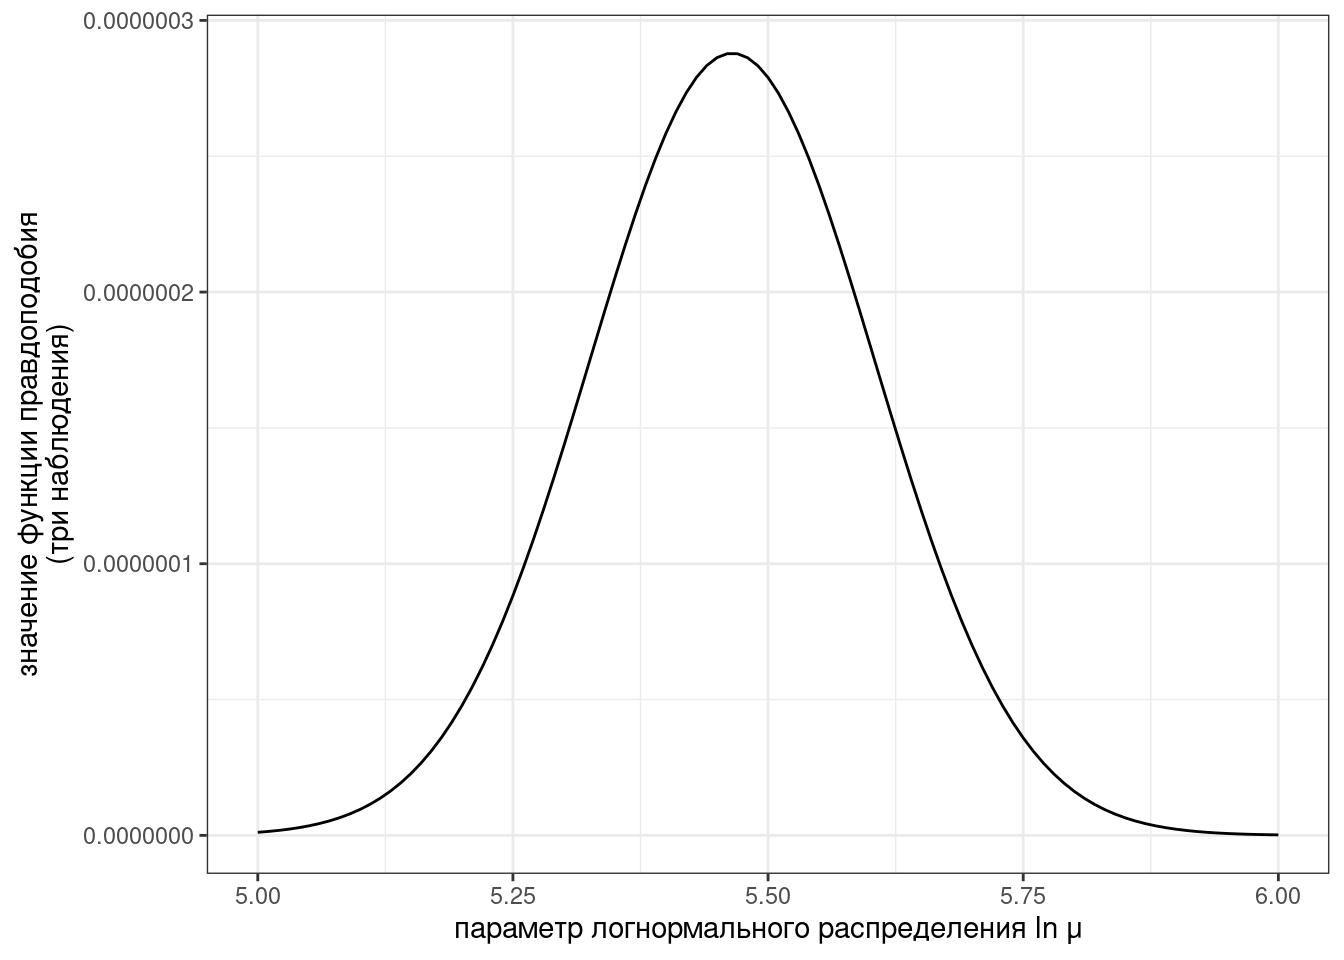
\includegraphics{da4l_files/figure-latex/unnamed-chunk-45-3.pdf}

Для простоты в начале я зафиксировал один из параметров логнормального распредления: лог стандартное отклонение. Конечно, это совсем необязательно делать: можно создать матрицу значений лог среднего и лог стандартного отклонения и получить для каждой ячейки матрицы значения функции правдоподобия.

\hypertarget{ux43cux435ux442ux43eux434-ux43cux430ux43aux441ux438ux43cux430ux43bux44cux43dux43eux433ux43e-ux43fux440ux430ux432ux434ux43eux43fux43eux434ux43eux431ux438ux44f-mle}{%
\section{Метод максимального правдоподобия (MLE)}\label{ux43cux435ux442ux43eux434-ux43cux430ux43aux441ux438ux43cux430ux43bux44cux43dux43eux433ux43e-ux43fux440ux430ux432ux434ux43eux43fux43eux434ux43eux431ux438ux44f-mle}}

Функция правдоподобия позволяет подбирать параметры распределения. Оценка параметров распределения при помощи функции максимального правдоподобия получила название метод максимального правдоподобия. Его я и использовал ранее для того, чтобы получить значения распределений для заданий из первого занятия:

\begin{itemize}
\tightlist
\item
  данные длительности американских гласных из \citep{hillenbrand95} и логнормальное распределение
\end{itemize}

\begin{Shaded}
\begin{Highlighting}[]
\NormalTok{fitdistrplus}\SpecialCharTok{::}\FunctionTok{fitdist}\NormalTok{(vowels}\SpecialCharTok{$}\NormalTok{dur, }\AttributeTok{distr =} \StringTok{\textquotesingle{}lnorm\textquotesingle{}}\NormalTok{, }\AttributeTok{method =} \StringTok{\textquotesingle{}mle\textquotesingle{}}\NormalTok{)}
\end{Highlighting}
\end{Shaded}

\begin{verbatim}
Fitting of the distribution ' lnorm ' by maximum likelihood 
Parameters:
         estimate  Std. Error
meanlog 5.5870359 0.005935135
sdlog   0.2423978 0.004196453
\end{verbatim}

\begin{itemize}
\tightlist
\item
  количество андийских слогов в словах и распределение Пуассона
\end{itemize}

\begin{Shaded}
\begin{Highlighting}[]
\NormalTok{andic\_syllables }\OtherTok{\textless{}{-}} \FunctionTok{read\_csv}\NormalTok{(}\StringTok{"https://raw.githubusercontent.com/agricolamz/2022\_da4l/master/data/andic\_syllables.csv"}\NormalTok{) }

\NormalTok{andic\_syllables }\SpecialCharTok{\%\textgreater{}\%} 
  \FunctionTok{filter}\NormalTok{(language }\SpecialCharTok{==} \StringTok{"Andi"}\NormalTok{) }\SpecialCharTok{\%\textgreater{}\%} 
  \FunctionTok{uncount}\NormalTok{(count) }\SpecialCharTok{\%\textgreater{}\%} 
  \FunctionTok{pull}\NormalTok{(n\_syllables) }\SpecialCharTok{\%\textgreater{}\%} 
\NormalTok{  fitdistrplus}\SpecialCharTok{::}\FunctionTok{fitdist}\NormalTok{(}\AttributeTok{distr =} \StringTok{\textquotesingle{}pois\textquotesingle{}}\NormalTok{, }\AttributeTok{method =} \StringTok{\textquotesingle{}mle\textquotesingle{}}\NormalTok{)}
\end{Highlighting}
\end{Shaded}

\begin{verbatim}
Fitting of the distribution ' pois ' by maximum likelihood 
Parameters:
       estimate Std. Error
lambda 2.782715 0.02128182
\end{verbatim}

\begin{itemize}
\tightlist
\item
  Есть и другие методы оценки параметров.
\item
  Метод максимального правдоподобия может быть чувствителен к размеру выборки.
\end{itemize}

\begin{rmdtask}
Отфильтруйте из
\href{https://raw.githubusercontent.com/agricolamz/2021_da4l/master/data/andic_syllables.csv}{данных
с количеством слогов в андийских языках} багвалинский и, используя метод
максимального правдоподобия, оцените для них параметры модели Пуассона.
\end{rmdtask}

\begin{rmdtask}
В работе {[}@coretta2016{]} собраны
\href{https://raw.githubusercontent.com/agricolamz/2021_da4l/master/data/Coretta_2017_icelandic.csv}{данные}
длительности исландских гласных. Отфильтруйте данные, оставив
односложные слова (переменная \texttt{syllables}) после придыхательного
(переменная \texttt{aspiration}), произнесенные носителем \texttt{tt01}
(переменная \texttt{speaker}) и постройте следующий график, моделируя
длительность гласных (переменная \texttt{vowel.dur}) нормальным и
логнормальным распределением. Как вам кажется, какое распределение лучше
подходит к данным? Докажите ваше утверждение, сравнив значения
правдоподобия.
\end{rmdtask}

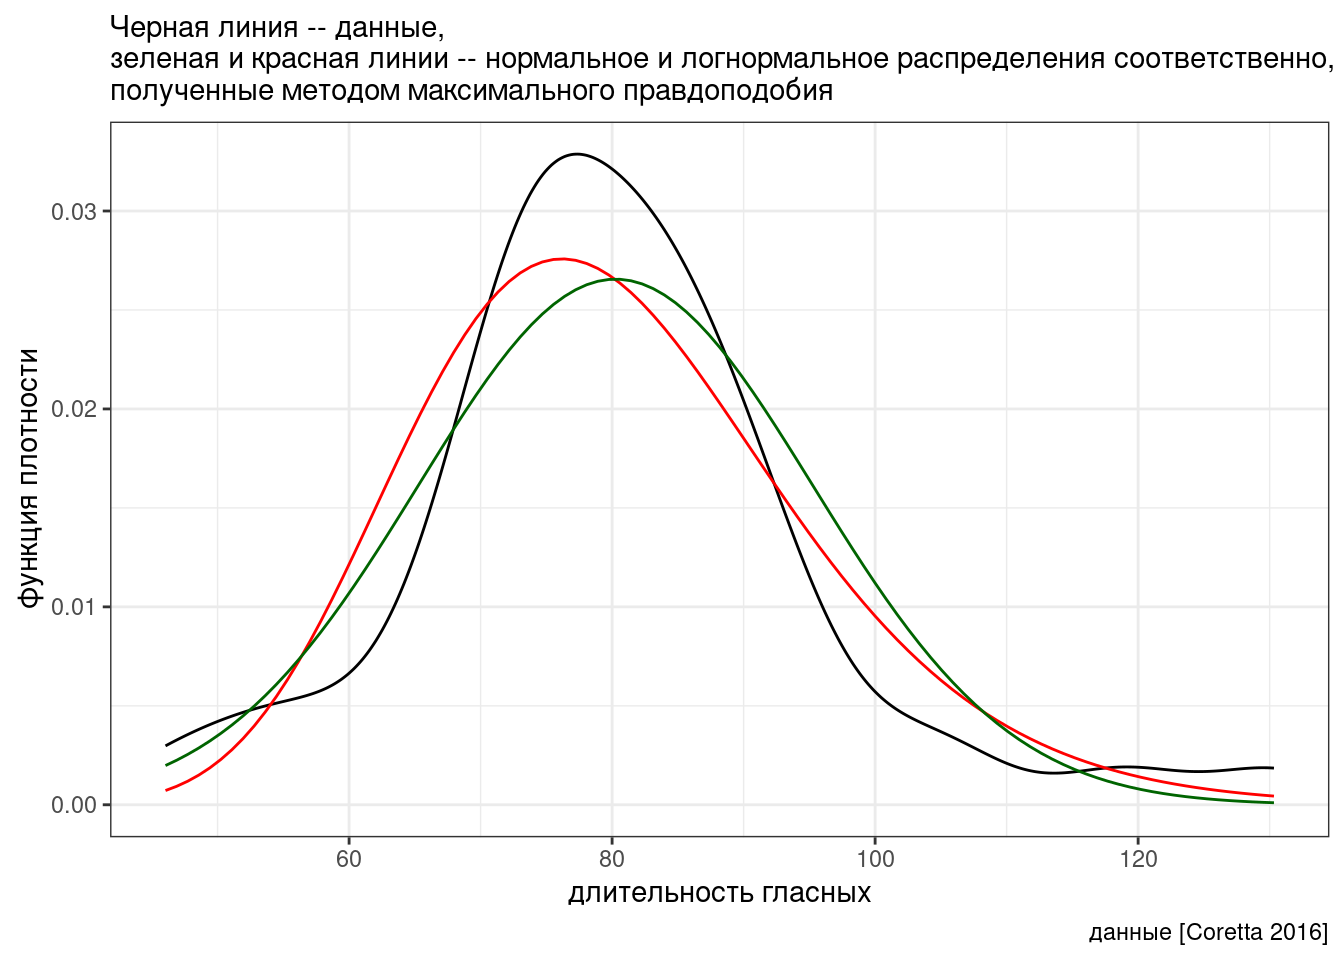
\includegraphics{da4l_files/figure-latex/unnamed-chunk-50-1.pdf}

\hypertarget{ux43bux43eux433ux43eux440ux438ux444ux43c-ux444ux443ux43dux43aux446ux438ux438-ux43fux440ux430ux432ux434ux43eux43fux43eux434ux43eux431ux438ux44f}{%
\section{Логорифм функции правдоподобия}\label{ux43bux43eux433ux43eux440ux438ux444ux43c-ux444ux443ux43dux43aux446ux438ux438-ux43fux440ux430ux432ux434ux43eux43fux43eux434ux43eux431ux438ux44f}}

Так как в большинстве случаев нужно найти лишь максимум функции правдоподобия, а не саму функцию \(\ell(x|\theta)\), то для облегчения подсчетов используют логорифмическую функцию правдоподобия \(\ln\ell(x|\theta)\): в результате, вместо произведения появляется сумма\footnote{Это просто свойство логарифмов: \texttt{log(5*5)\ =\ log(5)+log(5)}}:

\[\text{argmax}_\theta \prod \ell(\theta|x) = \text{argmax}_\theta \sum \ln\ell(\theta|x) \]

Во всех предыдущих примерах мы смотрели на 1-3 примера данных, давайте попробуем использовать функцию правдоподобия для большего набора данных.

\begin{rmdtask}
Представим, что мы проводим некоторый эксперимент, и у некоторых
участников все получается с первой попытки, а некоторым нужна еще одна
попытка или даже две. Дополните код функциями правдоподобия и
логорифмической функцией правдоподобия, чтобы получился график ниже.
\end{rmdtask}

\begin{Shaded}
\begin{Highlighting}[]
\FunctionTok{set.seed}\NormalTok{(}\DecValTok{42}\NormalTok{)}
\NormalTok{v }\OtherTok{\textless{}{-}} \FunctionTok{sample}\NormalTok{(}\DecValTok{0}\SpecialCharTok{:}\DecValTok{2}\NormalTok{, }\DecValTok{10}\NormalTok{, }\AttributeTok{replace =} \ConstantTok{TRUE}\NormalTok{)}

\FunctionTok{sapply}\NormalTok{(}\FunctionTok{seq}\NormalTok{(}\FloatTok{0.01}\NormalTok{, }\FloatTok{0.99}\NormalTok{, }\FloatTok{0.01}\NormalTok{), }\ControlFlowTok{function}\NormalTok{(p)\{}
\NormalTok{  ...}
\NormalTok{\}) }\OtherTok{{-}\textgreater{}}
\NormalTok{  likelihood}

\FunctionTok{sapply}\NormalTok{(}\FunctionTok{seq}\NormalTok{(}\FloatTok{0.01}\NormalTok{, }\FloatTok{0.99}\NormalTok{, }\FloatTok{0.01}\NormalTok{), }\ControlFlowTok{function}\NormalTok{(p)\{}
\NormalTok{  ...}
\NormalTok{\}) }\OtherTok{{-}\textgreater{}}
\NormalTok{  loglikelihood}

\FunctionTok{tibble}\NormalTok{(}\AttributeTok{p =} \FunctionTok{seq}\NormalTok{(}\FloatTok{0.01}\NormalTok{, }\FloatTok{0.99}\NormalTok{, }\FloatTok{0.01}\NormalTok{),}
\NormalTok{       loglikelihood,}
\NormalTok{       likelihood) }\SpecialCharTok{\%\textgreater{}\%} 
  \FunctionTok{pivot\_longer}\NormalTok{(}\AttributeTok{names\_to =} \StringTok{"type"}\NormalTok{, }\AttributeTok{values\_to =} \StringTok{"value"}\NormalTok{, loglikelihood}\SpecialCharTok{:}\NormalTok{likelihood) }\SpecialCharTok{\%\textgreater{}\%} 
  \FunctionTok{ggplot}\NormalTok{(}\FunctionTok{aes}\NormalTok{(p, value))}\SpecialCharTok{+}
  \FunctionTok{geom\_line}\NormalTok{()}\SpecialCharTok{+}
  \FunctionTok{geom\_vline}\NormalTok{(}\AttributeTok{xintercept =} \FloatTok{0.33}\NormalTok{, }\AttributeTok{linetype =} \DecValTok{2}\NormalTok{)}\SpecialCharTok{+}
  \FunctionTok{facet\_wrap}\NormalTok{(}\SpecialCharTok{\textasciitilde{}}\NormalTok{type, }\AttributeTok{scales =} \StringTok{"free\_y"}\NormalTok{, }\AttributeTok{nrow =} \DecValTok{2}\NormalTok{)}\SpecialCharTok{+}
  \FunctionTok{scale\_x\_continuous}\NormalTok{(}\AttributeTok{breaks =} \FunctionTok{c}\NormalTok{(}\DecValTok{0}\SpecialCharTok{:}\DecValTok{5}\SpecialCharTok{*}\FloatTok{0.25}\NormalTok{, }\FloatTok{0.33}\NormalTok{))}
\end{Highlighting}
\end{Shaded}

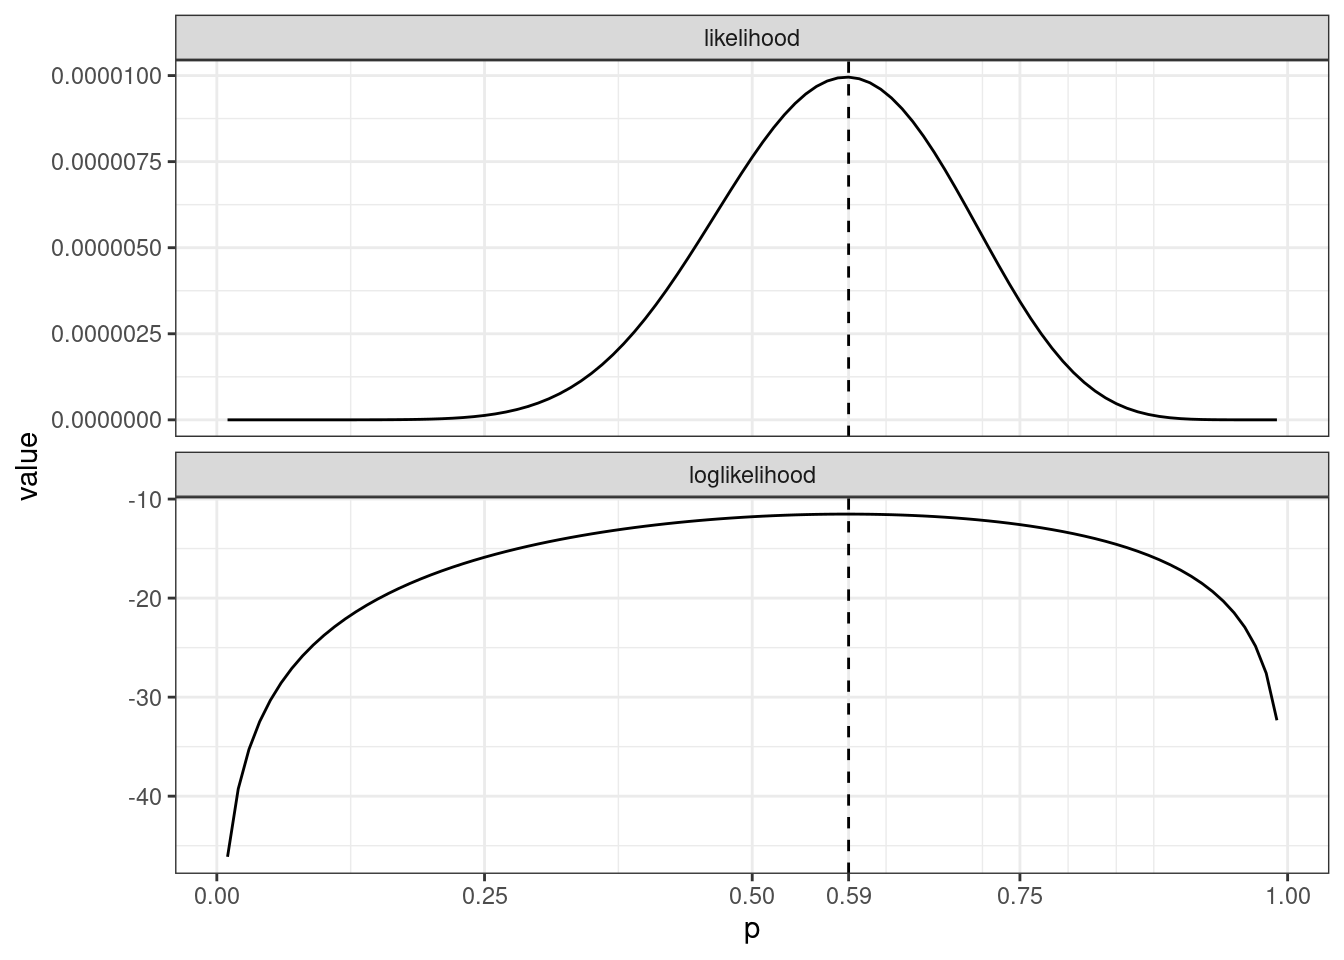
\includegraphics{da4l_files/figure-latex/unnamed-chunk-53-1.pdf}

  \bibliography{bibliography.bib}

\end{document}
